%%%%%%%%%%%%%%%%%%%%%%%%%%%%%%%%%%%%%%%%%%%%%%%%%%%%%%%%%%%%%%%%%%%%%%%%%%%%%%%%%%%%%%%%%%%%%%%%%%%%%%%%%%%%%%%%%%%%%%%%%%%%%%%%%%%%%%%%%%%%%%%%%%%%%%%%%%%%%%%%%%%%%%%
%%%%%%%%%%%%%%%%%%%%%%%%%%%%%%%%%%%%%%%%%%%%%%%%%%%%%%%%%%%%%%%%%%%%%%%%%%%%%%%%%%%%%%%%%%%%%%%%%%%%%%%%%%%%%%%%%%%%%%%%%%%%%%%%%%%%%%%%%%%%%%%%%%%%%%%%%%%%%%%%%%%%%%%
%%%%%%%%%%%%%%%%%%%%%%%%%%%%%%%%%%%%%%%%%%%%%%%%%%%%%%%%%%%%%%%%%%%%%%%%%%%%%%%%%%%%%%%%%%%%%%%%%%%%%%%%%%%%%%%%%%%%%%%%%%%%%%%%%%%%%%%%%%%%%%%%%%%%%%%%%%%%%%%%%%%%%%%
%%%%%%%%%%%%%%%%%%%%%%%%%%%%%%%%%%%%%%%%%%%%%%%%%%%%%%%%%%%%%%%%%%%%%%%%%%%%%%%%%%%%%%%%%%%%%%%%%%%%%%%%%%%%%%%%%%%%%%%%%%%%%%%%%%%%%%%%%%%%%%%%%%%%%%%%%%%%%%%%%%%%%%%
%%%%%%%%%%%%%%%%%%%%%%%%%%%%%%%%%%%%%%%%%%%%%%%%%%%%%%%%%%%%%%%%%%%%%%%%%%%%%%%%%%%%%%%%%%%%%%%%%%%%%%%%%%%%%%%%%%%%%%%%%%%%%%%%%%%%%%%%%%%%%%%%%%%%%%%%%%%%%%%%%%%%%%%
%%%%%%%%%%%%%%%%%%%%%%%%%%%%%%%%%%%%%%%%%%%%%%%%%%%%%%%%%%%%%%%%%%%%%%%%%%%%%%%%%%%%%%%%%%%%%%%%%%%%%%%%%%%%%%%%%%%%%%%%%%%%%%%%%%%%%%%%%%%%%%%%%%%%%%%%%%%%%%%%%%%%%%%
\FloatBarrier
\chapter{Interpretation}
\label{sec:Interpretation}
In order to interpret the result of the search in the context of supersymmetric models with almost mass degenerate charginos and neutralinos, sources of systematic uncertainties on the number of selected signal events must be identified and quantified.
The interpretation will then be done with statistical methods that allow for the exclusion of parts of the supersymmetric parameter space on a 95\% confidence level.

\section{Systematic uncertainties of simulated signal samples}
The systematic uncertainties on the number of signal events in the four signal regions are caused by uncertainties in the generation and simulation of signal events and the integrated luminosity of the considered data.

All systematic uncertainties are estimated for each signal model (cf. Section~\ref{sec:SignalSamples}) and each search bin separately.
In the following, the sources of systematic uncertainties are discussed and the range of the corresponding uncertainty is given.

\subsection*{Uncertainty on the theoretical cross section}
The theoretical cross sections of $\chipm\chimp$ and $\chipm\chiO$ production at a centre-of-mass energy of 8\tev are taken from~\cite{bib:SignalCrossSection_2012,bib:SignalCrossSection_2013}.
The corresponding theoretical uncertainties range between $4.5-12.1\%$.

\subsection*{Luminosity uncertainty}
The integrated luminosity recorded at CMS during the year 2012 is measured by counting of pixel clusters during the crossing of two bunches (zero-bias event).
A detailed explanation of this method and the corresponding total uncertainty of 2.6\% can be found in \cite{bib:CMS:Lumi_PAS}.

\subsection*{Uncertainty on the simulation of initial state radiation}
Initial state radiation affects the transverse momentum distribution of the 2-particle system, $\pt\left(p_1^{\mu} + p_2^{\mu} \right)$, in a 2-body decay.
Differences between data and simulation of ISR are taken into account by reweighting the simulated events, such that the simulated transverse momentum distribution matches the measured distribution in data. 
The weights and associated systematic uncertainties are determined in~\cite{bib:CMS:ISR_AN} by comparing simulated and observed \pt distributions of $Z$ and $\bar{t}t$ events.
These weights are applied to the simulated $\chipm\chimp$ and $\chipm\chiO$ events.
To account for the systematic uncertainties on the reweighting procedure, the event weights are varied up and down by up to 25\% according to~\cite{bib:CMS:ISR_AN} depending on the transverse momentum of the $\chi_1\chi_2$ system.
The resulting uncertainty on the ISR simulation is between $9.2-12.6\%$.

\subsection*{Uncertainty on the simulation of the trigger efficiency}
The HLTMonoCentralPFJet80\_PFMETnoMu105\_NHEF0p95 trigger with the higher MET threshold of 105\gev active in Run\,C and Run\,D during 2012 was not available in the simulated signal samples.
It is therefore emulated using HLT trigger information. 
More details on the emulation of this trigger can be found in Appendix~\ref{app:TriggerEmulation}.

The trigger uncertainty is assessed by comparing data-simulation differences of the trigger efficiency.
This uncertainty has been quantified within~\cite{bib:CMS:DT_Thesis,bib:CMS:DT_8TeV_AN} by comparing simulated and measured trigger turn-on curves and determining weights for simulated events such that simulated and observed turn-on curves are compatible.
These event weights are applied on the simulated signal samples in this analysis and lead to changes in the signal prediction of 1.9 to 4.4\%, which are taken as sytematic uncertainties.

\subsection*{Uncertainty on the jet energy scale}
The transverse momentum of all jets is corrected for non-uniformities in the energy response as a function of the jet $\eta$ and \pt and for data-simulation differences~\cite{bib:CMS:JME_PAS}.
The uncertainty on the jet energy scale (JES) is neatly described and quantified in~\cite{bib:CMS:JME_PAS}. 
It arises from uncertainties on the measured jet response in data including jet fragmentation, jet flavor composition, etc..
The JES correction is applied as a multiplicative factor on each jet's transverse momentum contained in an event.
The corresponding systematic uncertainty is assessed by an up- and downward variation of the correction factor within 1\,$\sigma$.
The resulting uncertainties are of minor importance and range between $0.4-3.1\%$.

\subsection*{Uncertainty on the jet energy resolution}
The jet energy resolution (JER) is smaller in simulation than in measured data (see Part~\ref{FIXME}). 
In order to take these differences into account, the simulated jet energy response is smeared to match the measured response.
The systematic uncertainty on the smearing factors is estimated in~\cite{bib:CMS:JME_PAS,bib:Kristin_Thesis}.
It covers the uncertainty on JER in data, including the JES uncertainty, uncertainties arising from out-of-cone showering etc.~\cite{bib:CMS:JME_PAS,bib:Kristin_Thesis}.
The resulting uncertainty on the signal efficiency in this study is between $0.1-2.0\%$ and therefore almost negligible.

\subsection*{Uncertainty on the simulation of the parton distribution functions}
The parton distribution function (PDF) used for the simulation of proton-proton collisions is provided by the \cteq group~\cite{Pumplin:2002vw} (see Section~\ref{FIXME} for more information about PDFs).
In~\cite{Pumplin:2002vw}, a detailed description of the determination of a parton distribution function and its uncertainties is given.
Practically, the estimation of the PDF uncertainty is done by the application of 44 different sets of event weights which take into account 22 different sources of uncertainties~\cite{Botje:2011sn,bib:PDF_practical} 
(up and down variations lead to a factor of 2).
The sources correspond inter alia to uncertainties in the single distributions of gluons, up/down-quarks, etc, with the gluon distribution being by far the largest source of uncertainty.
The resulting uncertainties on the signal efficiency for this search are between $2.6-6.8\%$.

\subsection*{Uncertainty of the pileup reweighting}
The distribution of the number of primary vertices in simulation is reweighted to match the measured distribution in data.
The distribution of the number of primary vertices in data is determined by the luminosity of each bunch-crossing times the proton-proton inelastic cross section which is 69.4\mb~\cite{bib:CMS:PileupUtilities}.
The uncertainty on the number of interactions thus consists of the uncertainty on the luminosity and the uncertainty on the cross section.
To cover both sources, a variation of the inelastic cross section by plus/minus 5\% is done according to the recommendation by~\cite{bib:CMS:PileupSysUnc}.

For most of the signal models and signal regions, the signal efficiency is only affected by less than 1\% by the pileup reweighting uncertainty.
If the statistical precision of the signal prediction in a specific search bin is low, the uncertainty can become significantly larger.
However, the search sensitivity is always driven by search bins with high signal content so that large values of this uncertainty have no effect on the overall search sensitivity.

\subsection*{Uncertainty on the simulation of the calorimeter isolation}
The uncertainty on the simulation of the calorimeter isolation \ecalo is estimated by comparing simulated and measured selection efficiencies of $\ecalo<5\gev$ in the fake enriched control sample \fakeCR.
The fake enriched control region is well suited for this estimation, because fake tracks are not correlated to the energy deposits in the calorimeters.
The selection efficiency in data is higher than in simulation in both \pt bins of $30-50\gev$ and $50-\infty\gev$.
This difference between data and simulation is taken as systematic uncertainty, resulting in uncertainties of 12.1\% and 3.0\%.

\subsection*{Uncertainty on the simulation of missing middle/inner hits}
The uncertainty on the simulation of the number of missing inner and middle hits is assessed by comparing the probability in simulation and data of passing the selection requirements of $N_{\text{miss}}^{\text{middle/inner}}=0$
of a candidate track in the muon-veto inverted control region. 
This control region is particularly suitable because muons are not expected to have intrinsic sources of missing hits, as \eg pions or electrons have.
Pions can interact nuclearly with the tracker material and electrons can have sizable radiative losses, such that both can change direction or don't deposit energy in a tracker layer.
For muons, on the other hand, sources of missing inner and middle hits are mainly algorithmic~\cite{bib:CMS:DT_Thesis,bib:CMS:DT_8TeV_AN}, 
making them very similar to the algorithmic sources of missing inner/middle hits for chargino tracks.

The uncertainty is estimated as the observed difference of the cut selection efficiency of $N_{\text{miss}}^{\text{middle/inner}}=0$ in data and simulation.
The selection efficiency is always higher in simulation, resulting in systematic uncertainties of around 3.5\% for the simulation of $N_{\text{miss}}^{\text{inner}}=0$ and around 2.2\% for $N_{\text{miss}}^{\text{middle}}=0$.
The uncertainties are of very similar size in the signal regions with different \pt.
No \ias dependence is considered.

\subsection*{Uncertainty on the simulation of \ias}
An uncertainty on the simulation of \ias needs to be estimated in order to account for possible data-simulation differences for highly ionising particles.
The estimation of the \ias uncertainty is done following the methodology in~\cite{bib:CMS:HSCP_8TeV,bib:CMS:HSCP_8TeV_AN}.
The \ias uncertainty can be assessed by comparing data and simulation differences of slow protons.
Slow protons are highly ionising and can thus be used to determine the uncertainty in the high \ias region.

In order to select slow protons, high quality tracks with a momentum smaller than 2.5\gev are selected.
The \ias versus momentum distribution for the selected tracks is shown in Fig.~\ref{fig:IasVsMomentum}.
\begin{figure}[!h]
  \centering 
  \begin{tabular}{c}
    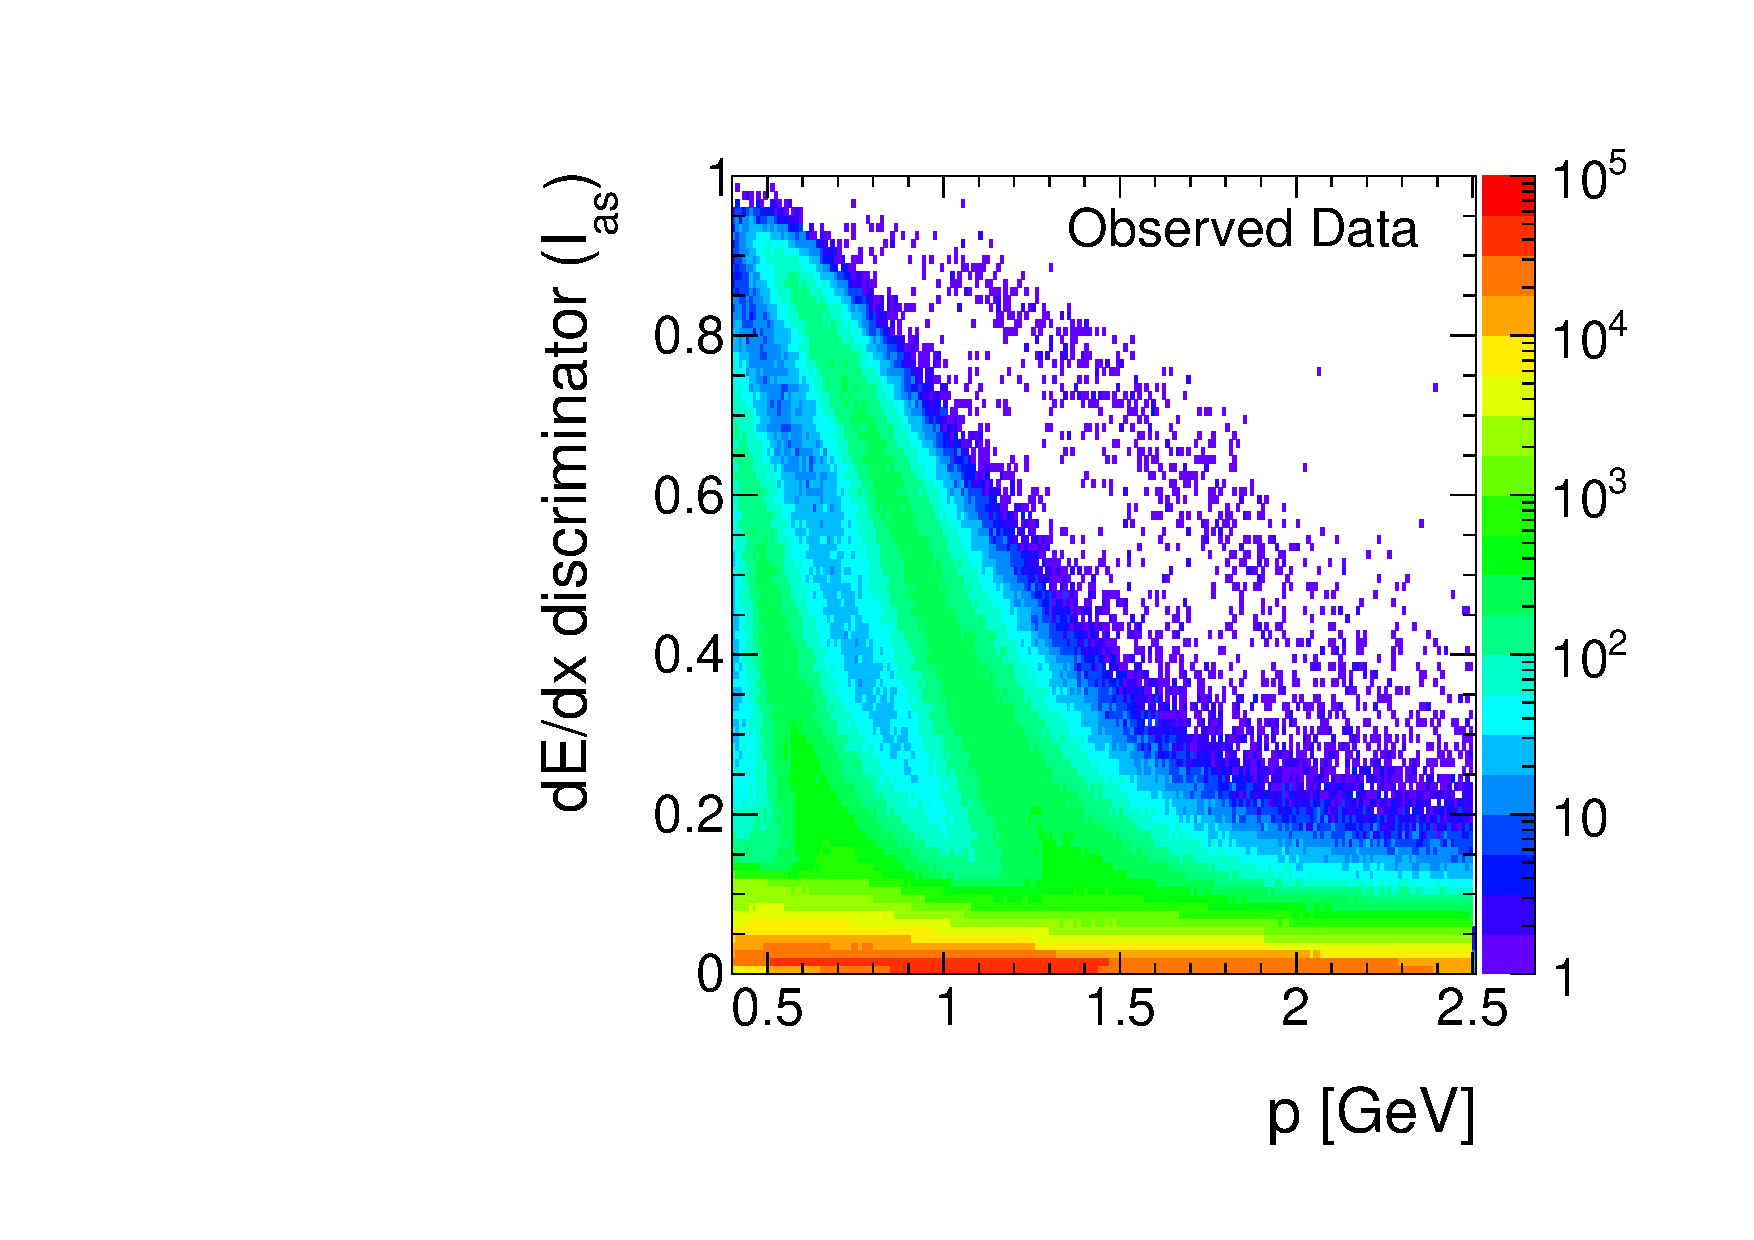
\includegraphics[width=0.49\textwidth]{figures/analysis/Interpretation/IasP_Data.pdf} 
    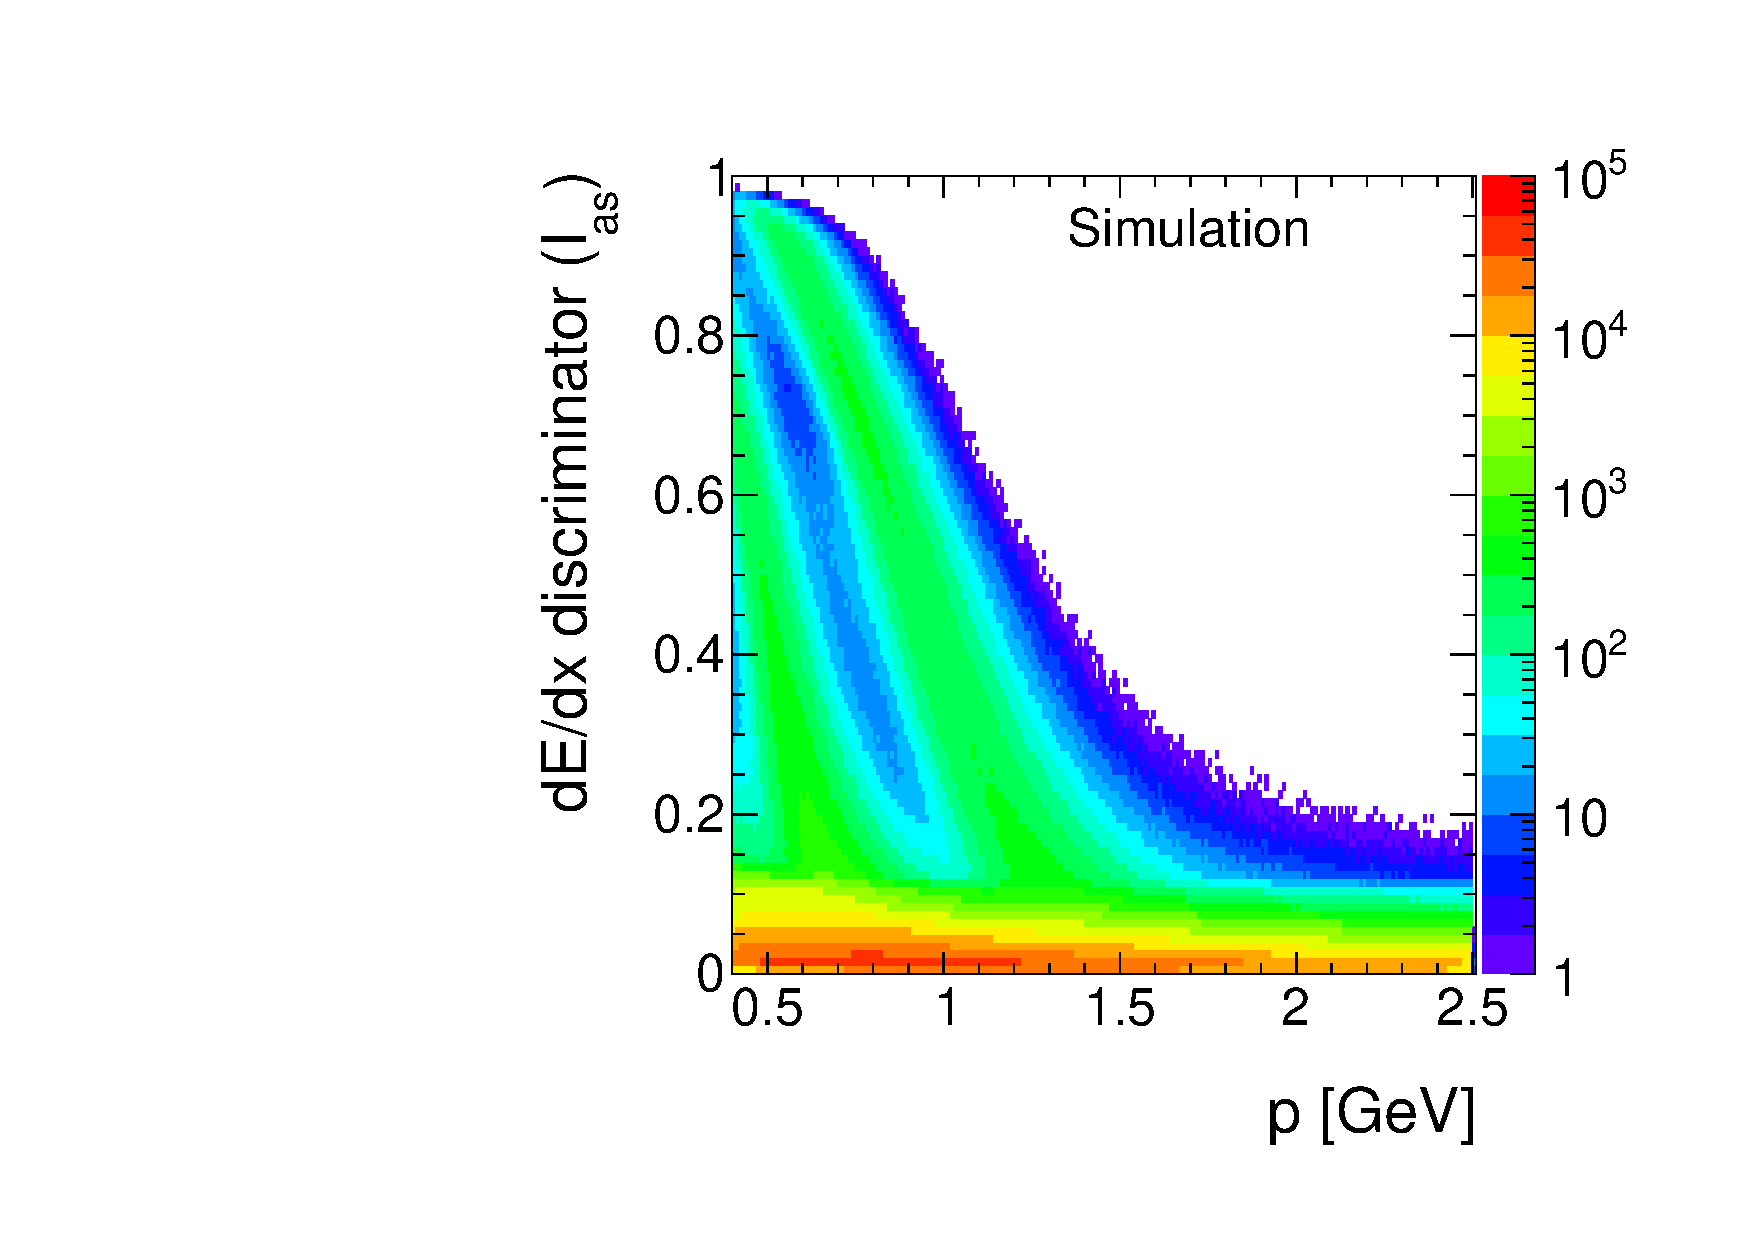
\includegraphics[width=0.49\textwidth]{figures/analysis/Interpretation/IasP_MC.pdf}
  \end{tabular}
  \caption{\ias versus momentum for good quality tracks with at least eight hits in observed data (left) and simulation (right).}
  \label{fig:IasVsMomentum}
\end{figure} 
The kaon and proton line are visible in both datasets. 
The deuteron line is only visible in data, as deuteron's are not simulated.
Two different slices in the momentum are extracted where the proton line is contained: p between $0.80-0.85\gev$ and $0.95-1.00\gev$.
A Gaussian function is fitted to the proton peak and the maximum difference of the mean of the fitted Gaussian between simulation and observed data is taken as systematic uncertainty.
The \ias distribution for the two momentum ranges with the Gaussian fit is depicted in Fig.~\ref{fig:IasSlowProtons}.
\begin{figure}[!h]
  \centering 
  \begin{tabular}{c}
    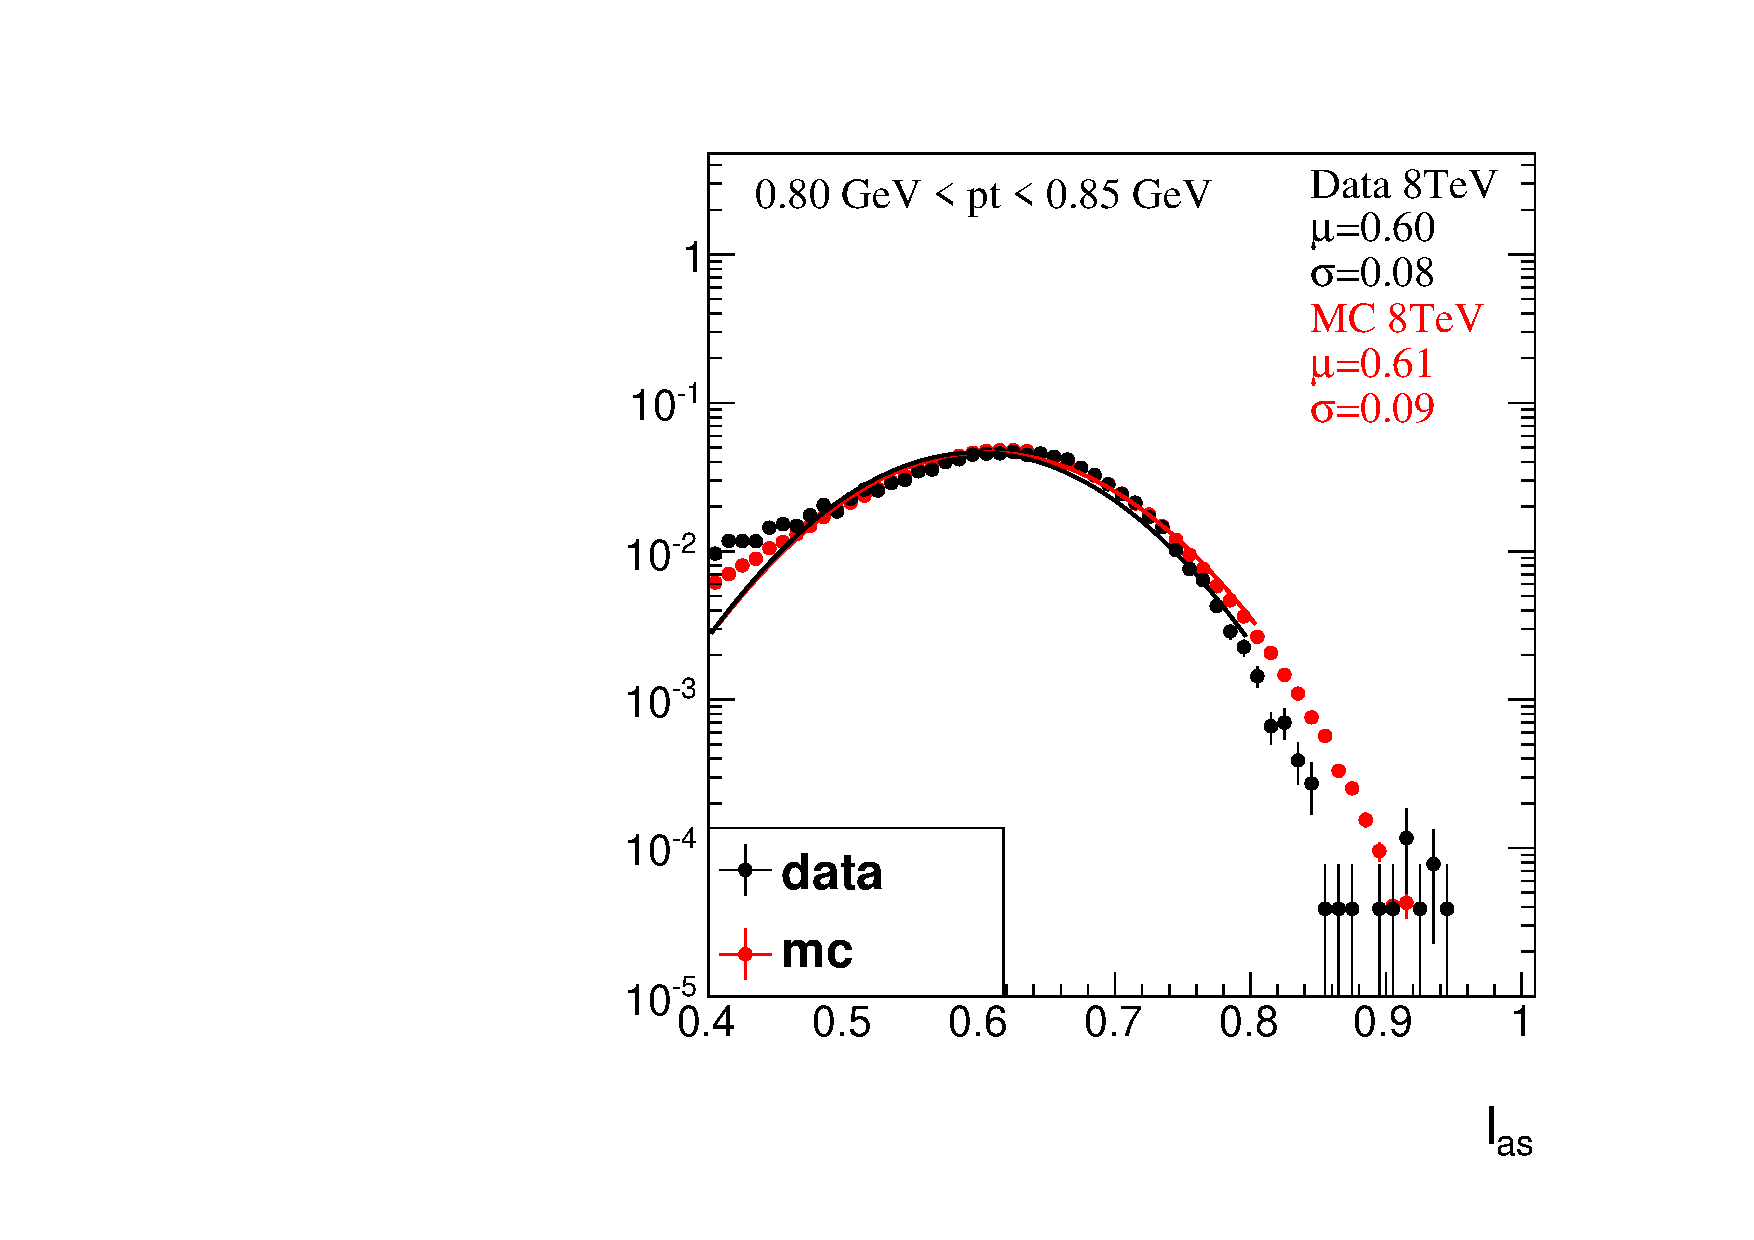
\includegraphics[width=0.49\textwidth]{figures/analysis/Interpretation/hIas_analysis_2015_11_30_ForThesis_ptmin0p80_ptmax0p85.pdf} 
    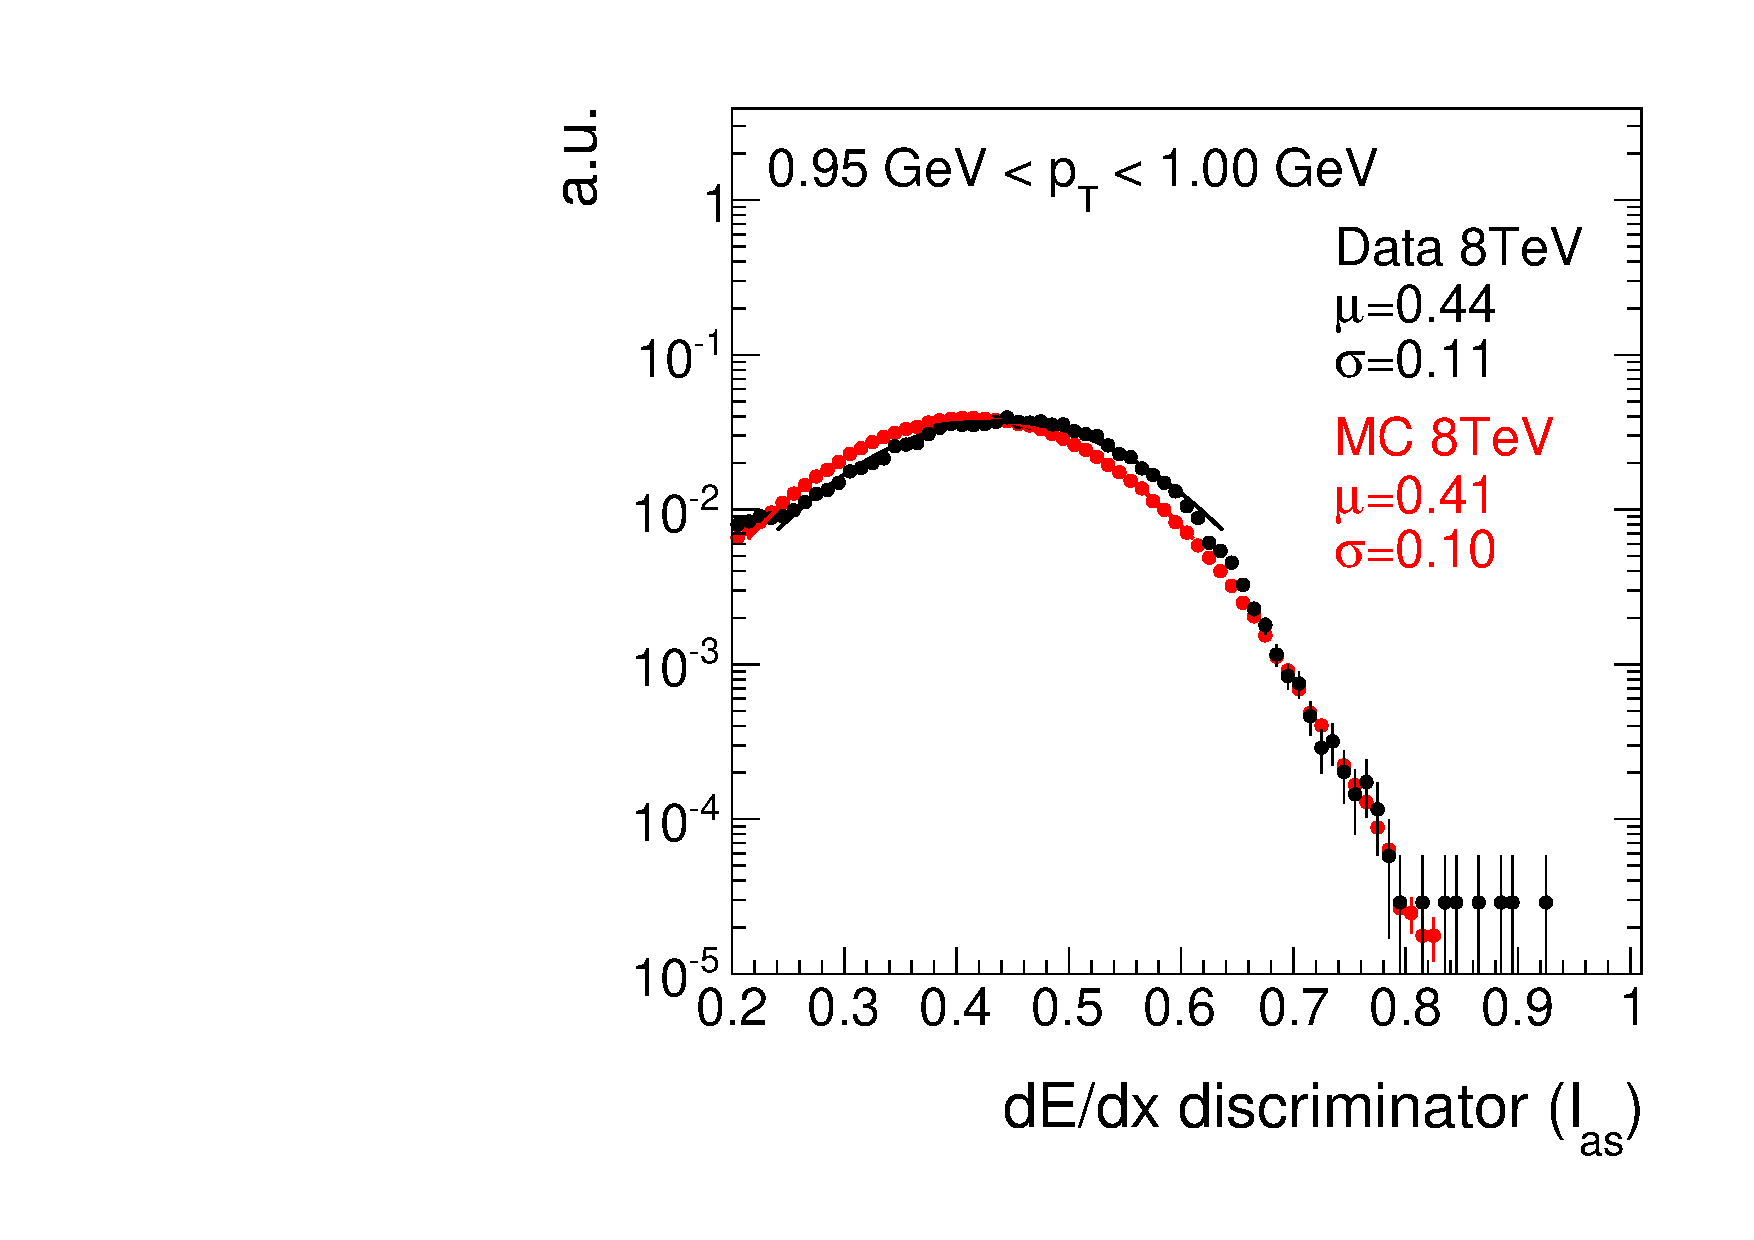
\includegraphics[width=0.49\textwidth]{figures/analysis/Interpretation/hIas_analysis_2015_11_30_ForThesis_ptmin0p95_ptmax1p0.pdf}
  \end{tabular}
  \caption{\ias distribution for slow protons in simulation and observed data for a momentum range of $0.80-0.85\gev$ (left) and $0.95-1.00\gev$ (left).
           For the momentum range of $0.80-0.85\gev$, the proton line is contained between \ias values of $0.4-0.8$, whereas for the momentum range of $0.95-1.00\gev$, the proton line \ias lies between $0.2-0.6$.  }
  \label{fig:IasSlowProtons}
\end{figure} 
The systematic uncertainty is estimated to a value of 6\%.
%The size of the systematic uncertainty is also expected to cover the data-simulation difference for minimal ionisation.


\subsection*{Uncertainty on the simulation of the track reconstruction efficiency}
One final source of uncertainty is the simulation of the track reconstruction efficiency.
Possible differences of the reconstruction efficiency in simulation and data can lead to a different signal acceptance.
Differences in the track reconstruction efficiency are especially expected for short tracks.
Therefore, a worst case estimation is done, comparing the track reconstruction efficiency in data and simulation for tracks with only three hits.

In simulation and observed data, well reconstructed muon tracks are selected and all hits after the third hit are removed.
Afterwards the full track reconstruction is performed again.
The relative difference of this track reconstruction efficiency in data and simulation is taken as systematic uncertainty. %($\epsilon = N_{\text{recon. trk matched to muon trk}}/N_{\text{selected muon trks}}$) 
The track reconstruction efficiency is higher in simulation than in data and results in uncertainties between $4.6-6.0\%$.\\


\subsection*{Summary of systematic uncertainties on the simulated signal samples}
All systematic uncertainties are estimated for all simulated signal samples and in each of the four signal regions.
An overview of the range of the uncertainties is given in Table~\ref{tab:SignalSysUnc}.

\renewcommand{\arraystretch}{1.5}
\begin{table}[!h] 
\centering
\caption{Ranges of systematic uncertainties on the simulated signal samples. Min and Max correspond to variations between different signal samples and search bins.}
\label{tab:SignalSysUnc}
\begin{tabular}{|l|c|c|}  
\multicolumn{3}{c}{} \\
\toprule
Uncertainty                             &Min [\%]           &Max [\%]           \\ 
\midrule
Theoretical x-section                   &4.5                &12.1               \\
Luminosity                              &2.6                &2.6                \\
Simulation of ISR                       &9.2                &12.6               \\ 
Simulation of trigger efficiency        &1.9                &4.4                \\ 
JES                                     &0.4                &3.1                \\ 
JER                                     &0.1                &2.0                \\ 
Simulation of PDF                       &2.6                &6.8                \\ 
Pileup reweighting                     &0.0                &16.0               \\ 
Simulation of calorimeter isolation     &3.0                &12.1               \\ 
Simulation of missing middle hits       &2.2                &2.2                \\ 
Simulation of missing inner hits        &3.3                &3.7                \\ 
Simulation of \ias                      &6.0                &6.0                \\ 
Simulation of track reconstruction efficiency    &4.6                &6.0                \\ 
\bottomrule
\multicolumn{3}{c}{} \\
\end{tabular}  
\end{table} 

In order to avoid an overestimation of the systematic uncertainties due to limited sizes of the samples (especially for low lifetimes like 1\cm), the corresponding signal sample with longer lifetime (100\cm) is used instead for determining the systematic uncertainty.
This is possible for uncertainty sources, where the size is not affected by the lifetime of the chargino, including ISR, trigger efficiency, JES, JER, and PDF uncertainties.

It can be seen, that major uncertainties are the simulation of the initial state radiation, of the calorimeter isolation, and of \ias.
The high maximum value of the pileup uncertainty is caused by limited statistical precision.

The systematic uncertainties on the simulated signal samples are considered as fully correlated among the four signal regions.

%%%%%%%%%%%%%%%%%%%%%%%%%%%%%%%%%%%%%%%%%%%%%%%%%%%%%%%%%%%%%%%%%%%%%%%%%%%%%%%%%%%%%%%%%%%%%%%%%%%%%%%%%%%%%%%%%%%%%%%%%%%%%%%%%%%%%%%%%%%%%%%%%%%%%%%%%%%%%%%%%%%%%%%
%%%%%%%%%%%%%%%%%%%%%%%%%%%%%%%%%%%%%%%%%%%%%%%%%%%%%%%%%%%%%%%%%%%%%%%%%%%%%%%%%%%%%%%%%%%%%%%%%%%%%%%%%%%%%%%%%%%%%%%%%%%%%%%%%%%%%%%%%%%%%%%%%%%%%%%%%%%%%%%%%%%%%%%
\section{Statistical Methods/ Limit setting}

This section is a small interlude to briefly introduce the methods and techniques that are used to exclude theoretical models with the results of this search.
For a detailed and pedagogical introduction to the methods, the reader is referred to~\cite{bib:Ott_Thesis}.

In this analysis, the exclusion of the underlying theoretical model is achieved with the \CLs method~\cite{bib:CLS_1999,bib:CLS_2000,bib:CLS_2002}.
A model is considered as excluded at a 95\% confidence level if \CLs is smaller than 5\%.
The \CLs method was developed for the Higgs searches at LEP in order not to overestimate the exclusion power of a result if an  under-fluctuation of the background expectation occurs.
\CLs is defined as the confidence level of the background plus signal hypothesis divided by the confidence level of the background only hypothesis
\begin{equation*}
\CLs = \frac{\CLsb}{\CLb}.
\end{equation*}
The confidence level CL is defined as the probability of obtaining less than or equal the number of observed events P($n\leq n_{\text{obs}}$) for a given background (or background+signal) hypothesis.
In general, the considered distribution can be any test statistics $Q$ and is not necessarily the distribution of the number of events.
However, For Poissonian statistics it leads to the following expressions for \CLsb and \CLb for one signal region
\begin{equation*}
\begin{split}
\CLsb &= \text{Poisson}\left( n\leq n_{\text{obs}} |\lambda = b+\mu\cdot s   \right),\\
\CLb  &= \text{Poisson}\left( n \leq n_{\text{obs}} |\lambda = b   \right),
\end{split}
\end{equation*}
where $\lambda$ is the mean of the Poisson distribution and the signal strength $\mu$ is the measure for the size of the signal cross section.

Systematic uncertainties are included by varying the background expectation $b$ and the signal expectation $\mu\cdot s$ according to a predefined probability density function (pdf).
For one Gaussian distributed source of systematic uncertainty on the background, this leads to the following expressions for \CLsb and \CLb
\begin{equation*}
\begin{split}
\CLsb &= \text{Poisson}\left( n \leq n_{\text{obs}} |\lambda = b \cdot (1+\delta_b)+\mu\cdot s   \right) \text{Gauss}\left(\delta_b|\text{mean}=0, \sigma = \sigma_b\right),\\
\CLb  &= \text{Poisson}\left( n \leq n_{\text{obs}} |\lambda = b \cdot (1+\delta_b)   \right) \text{Gauss}\left(\delta_b|\text{mean}=0, \sigma = \sigma_b\right),
\end{split}
\end{equation*}
These expressions can be generalised for more than one signal region and more than one systematic uncertainty~\cite{bib:Ott_Thesis}.
In case of multiple signal regions, the distribution of the systematic uncertainties becomes a multi-dimensional probability density function that takes the covariance matrix of the systematic uncertainties in different signal regions into account.
In order to get rid of the nuisance parameters $\delta_s$ and $\delta_b$, the expression for \CLs is integrated over all possible values of $\delta_{s/b}$.
This integration is generally not solvable analytically, but is calculated with pseudo data drawn from the pdf and inserted into the Poisson distribution.

In this search, the systematic uncertainties on the background and the signal yields as well as the statistical uncertainty on the fake background are modelled with log-normal distributions, 
whereas the statistical uncertainties on the leptonic background are modelled using gamma distributions.
A log-normal distribution is used instead of a normal distribution to ensure that the prediction cannot become negative.
The gamma distribution is well suited for statistical uncertainties arising from very limited statistical precision in control regions or in simulated samples that are used for the background estimation~\cite{bib:CMS:Combine}.

Correlations between systematic uncertainties on the background expectation in different search bins are assumed as shown in Table~\ref{tab:BkgSysUncCorr}.
The systematic uncertainties on the expected signal yields are considered fully correlated across search bins.

The exclusion limits are derived according to the above presented methodology using the \textit{Combine} framework~\cite{bib:CMS:Combine} which was developed for the Higgs searches at CMS.
\renewcommand{\arraystretch}{1.5}
\begin{table}[!h] 
\centering
\caption{Correlation of systematic and statistical uncertainties between the four different signal regions.}
\label{tab:BkgSysUncCorr}
\begin{tabularx}{\textwidth}{|X|X|X|X|X|}  
\multicolumn{5}{c}{} \\
\toprule 
                                        & Fakes                        & Taus                          & Electrons                      & Muons                       \\ 
\midrule
Statistical uncertainty                 &0\% correlated                & 100\% for same bins in \ias   & 0\% correlated                 & 100\% for same bins in \ias \\
\midrule
Leptonic scale factor uncertainty       & \makecell[c]{-}              & 100\% for same bins in \ias   & 100\% for same bins in \ias    & 100\% for same bins in \ias \\
\midrule
Fake rate  uncertainty                  & 100\% for same bins in \ias  &  \makecell[c]{-}              &  \makecell[c]{-}                &  \makecell[c]{-}           \\
\midrule
\ias uncertainty                         &0\% correlated                & 100\% for same bins in \pt    & 100\% for same bins in \pt     &  100\% for same bins in \pt \\
\bottomrule
\multicolumn{5}{c}{} \\
\end{tabularx}  
\end{table} 

%%%%%%%%%%%%%%%%%%%%%%%%%%%%%%%%%%%%%%%%%%%%%%%%%%%%%%%%%%%%%%%%%%%%%%%%%%%%%%%%%%%%%%%%%%%%%%%%%%%%%%%%%%%%%%%%%%%%%%%%%%%%%%%%%%%%%%%%%%%%%%%%%%%%%%%%%%%%%%%%%%%%%%%
%%%%%%%%%%%%%%%%%%%%%%%%%%%%%%%%%%%%%%%%%%%%%%%%%%%%%%%%%%%%%%%%%%%%%%%%%%%%%%%%%%%%%%%%%%%%%%%%%%%%%%%%%%%%%%%%%%%%%%%%%%%%%%%%%%%%%%%%%%%%%%%%%%%%%%%%%%%%%%%%%%%%%%%
\FloatBarrier
\section{Exclusion limits}
\label{sec:ExclusionLimits}

The presented search for highly ionising, short tracks is interpreted in the context of SUSY models with almost mass degenerate wino-like charginos and neutralinos.
As explained in the previous section, the exclusion is done with the help of the \CLs method.
Two direct production channels are taken into account: chargino pair production and chargino neutralino production. 
The corresponding cross sections can be found in Table~\ref{tab:SignalCrossSections}.

In total, 37 different lifetimes from $\ctau=1-10000\cm$ for each mass point ($100-600\gev$) are considered, leading to 37 different exclusion limits.
Four exemplary exclusion limits are shown in Fig.~\ref{fig:1dLimits}, the full set of exclusion limits can be found in Appendix~\ref{app:ExlusionLimits}.

\begin{figure}[!h]
  \centering 
  \vspace{70pt}
  \begin{tabular}{c}
    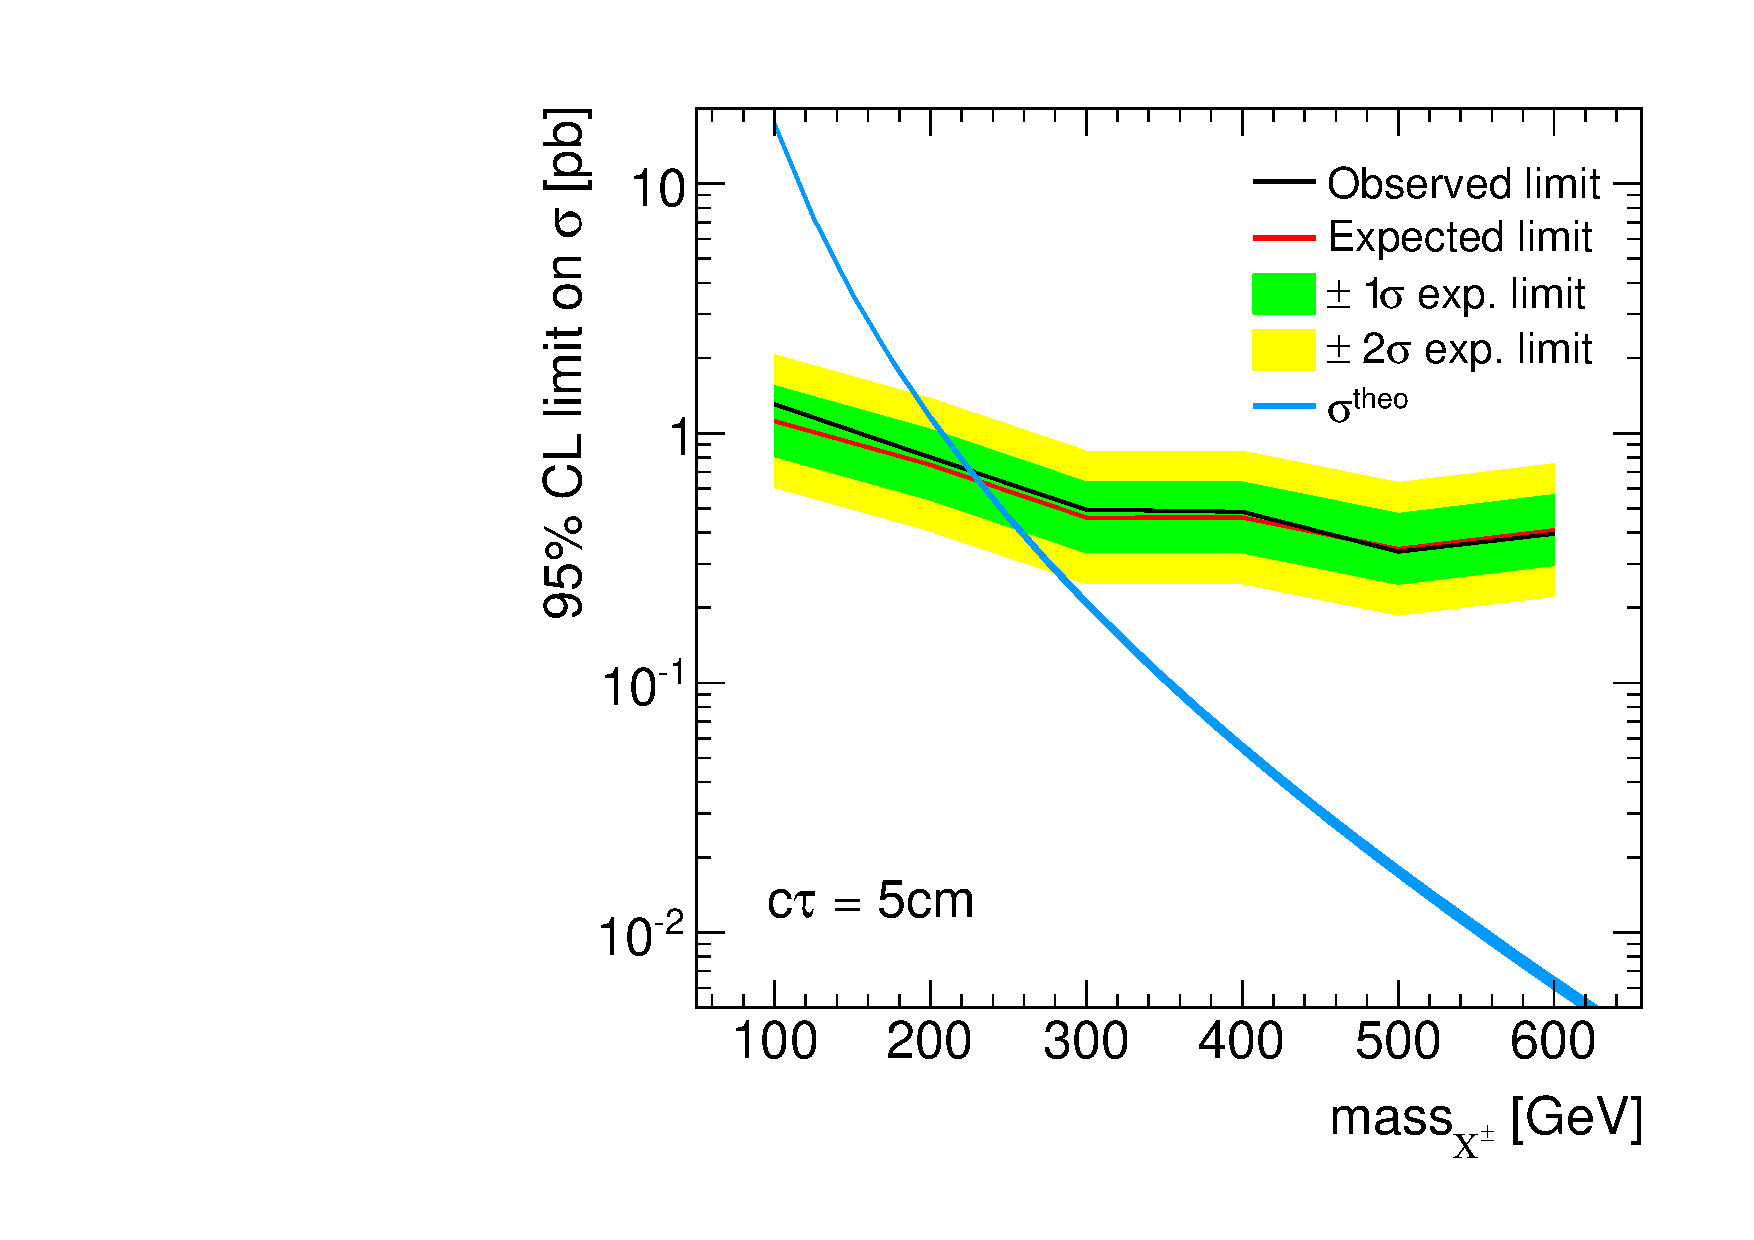
\includegraphics[width=0.49\textwidth]{figures/analysis/Interpretation/ExclusionLimits/LimitPlot_ctau5cm.pdf} 
    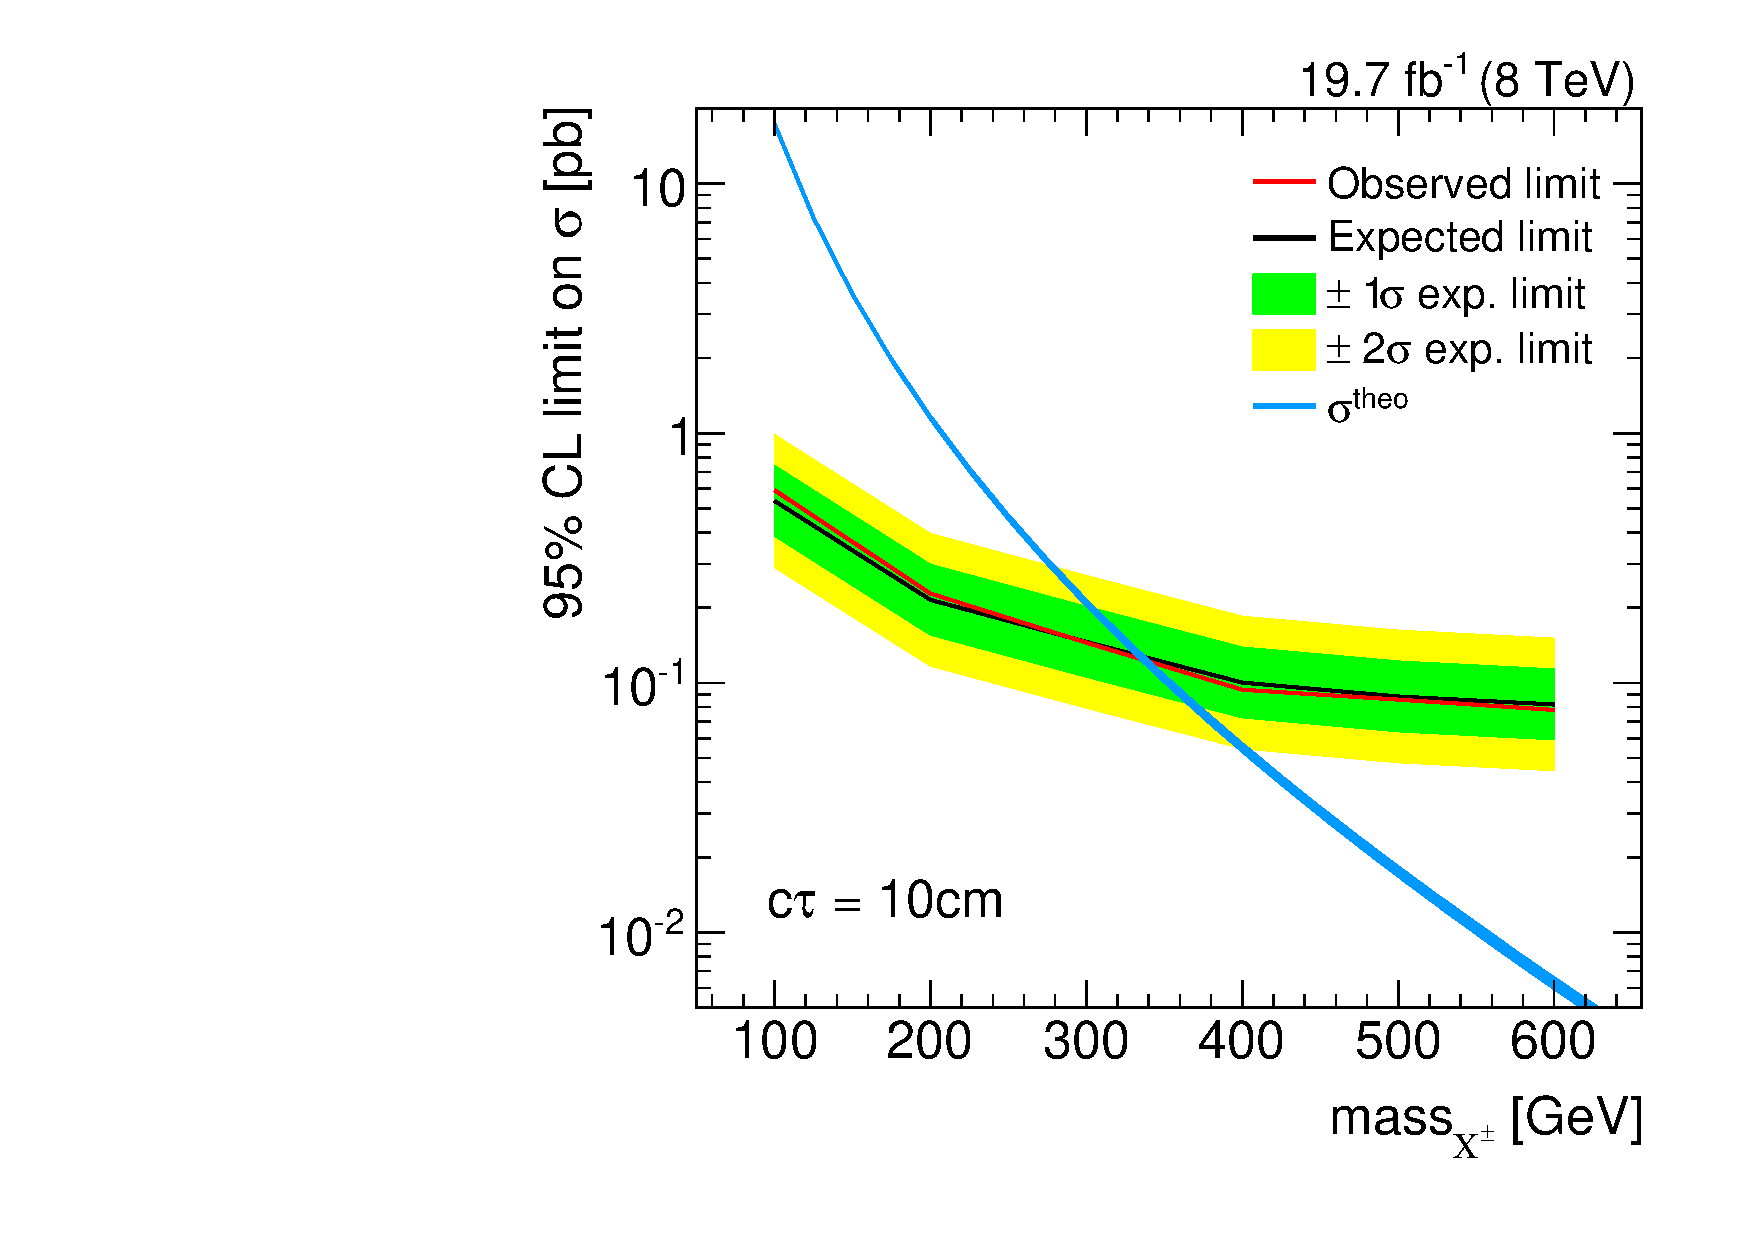
\includegraphics[width=0.49\textwidth]{figures/analysis/Interpretation/ExclusionLimits/LimitPlot_ctau10cm.pdf} \\
    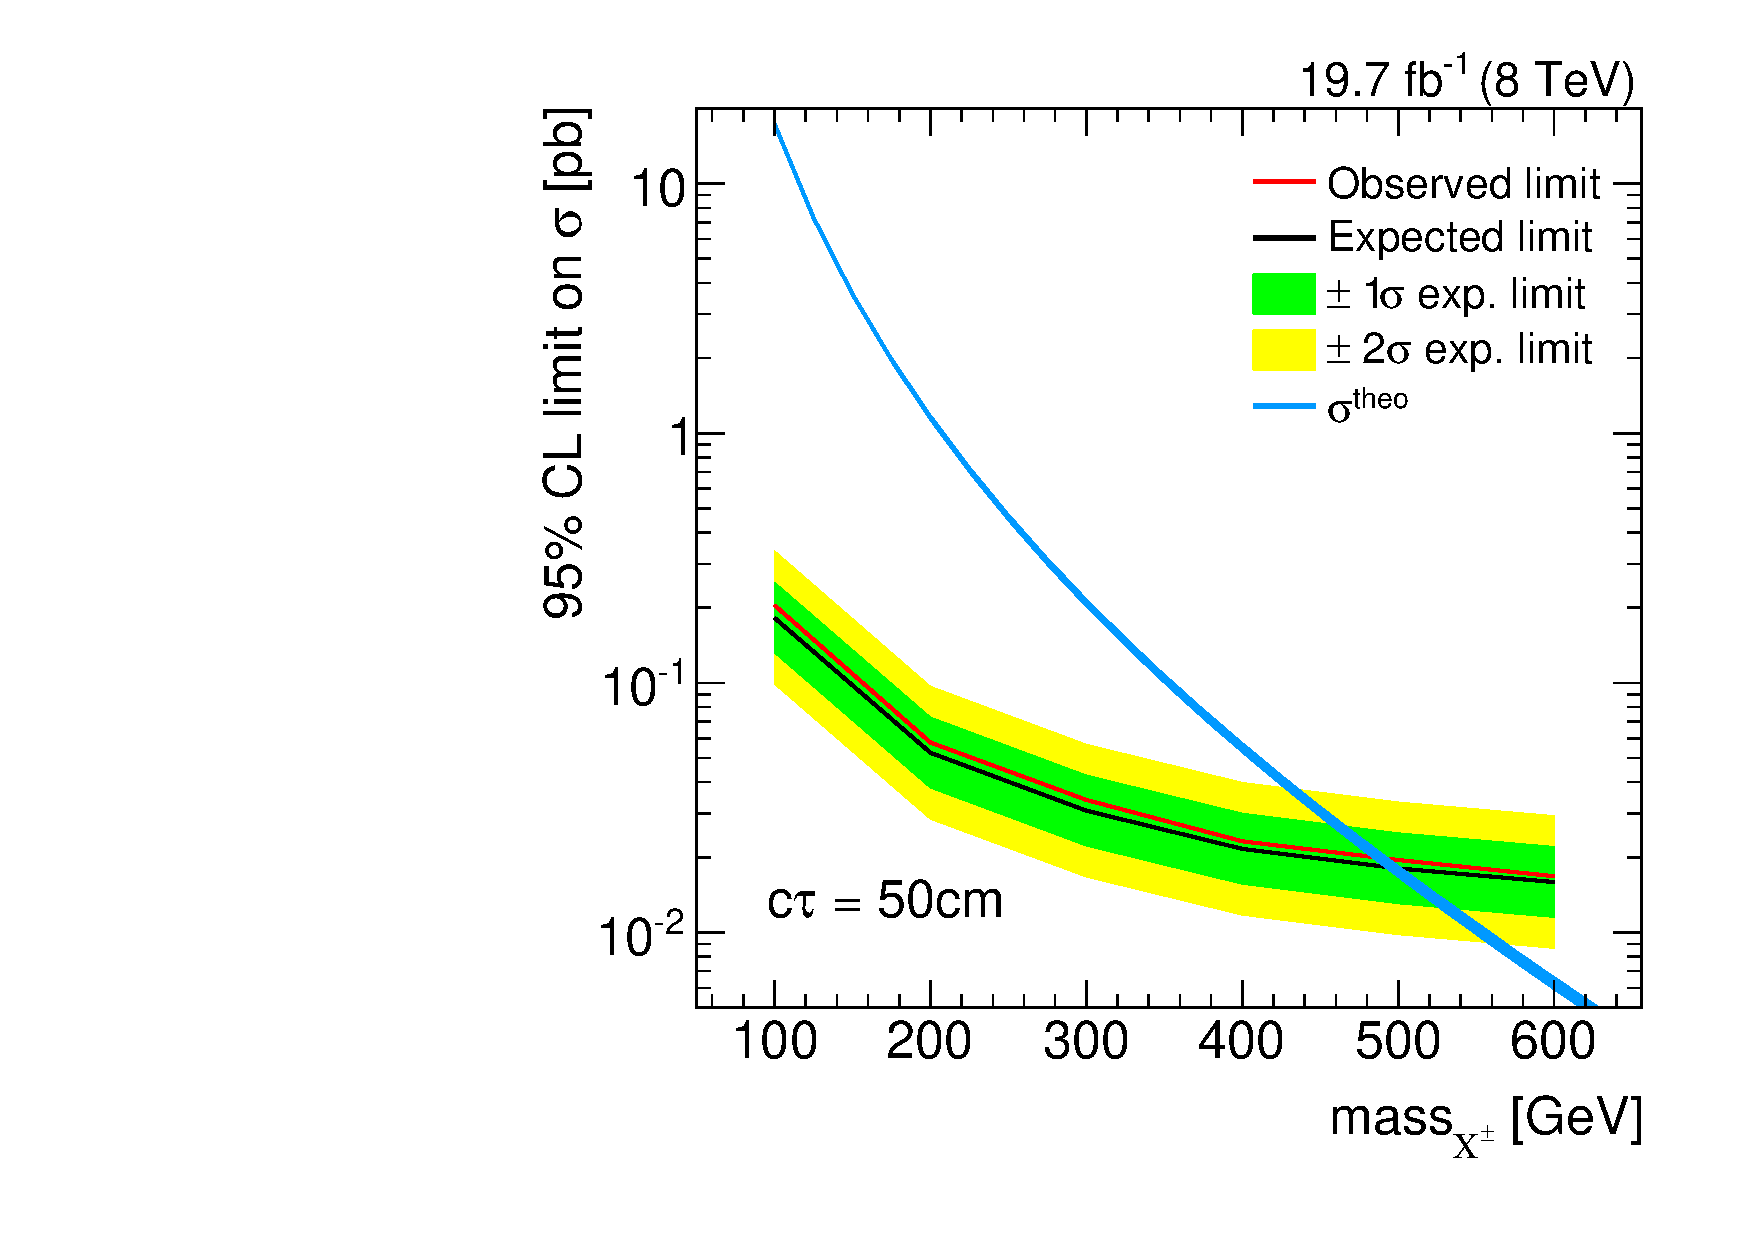
\includegraphics[width=0.49\textwidth]{figures/analysis/Interpretation/ExclusionLimits/LimitPlot_ctau50cm.pdf} 
    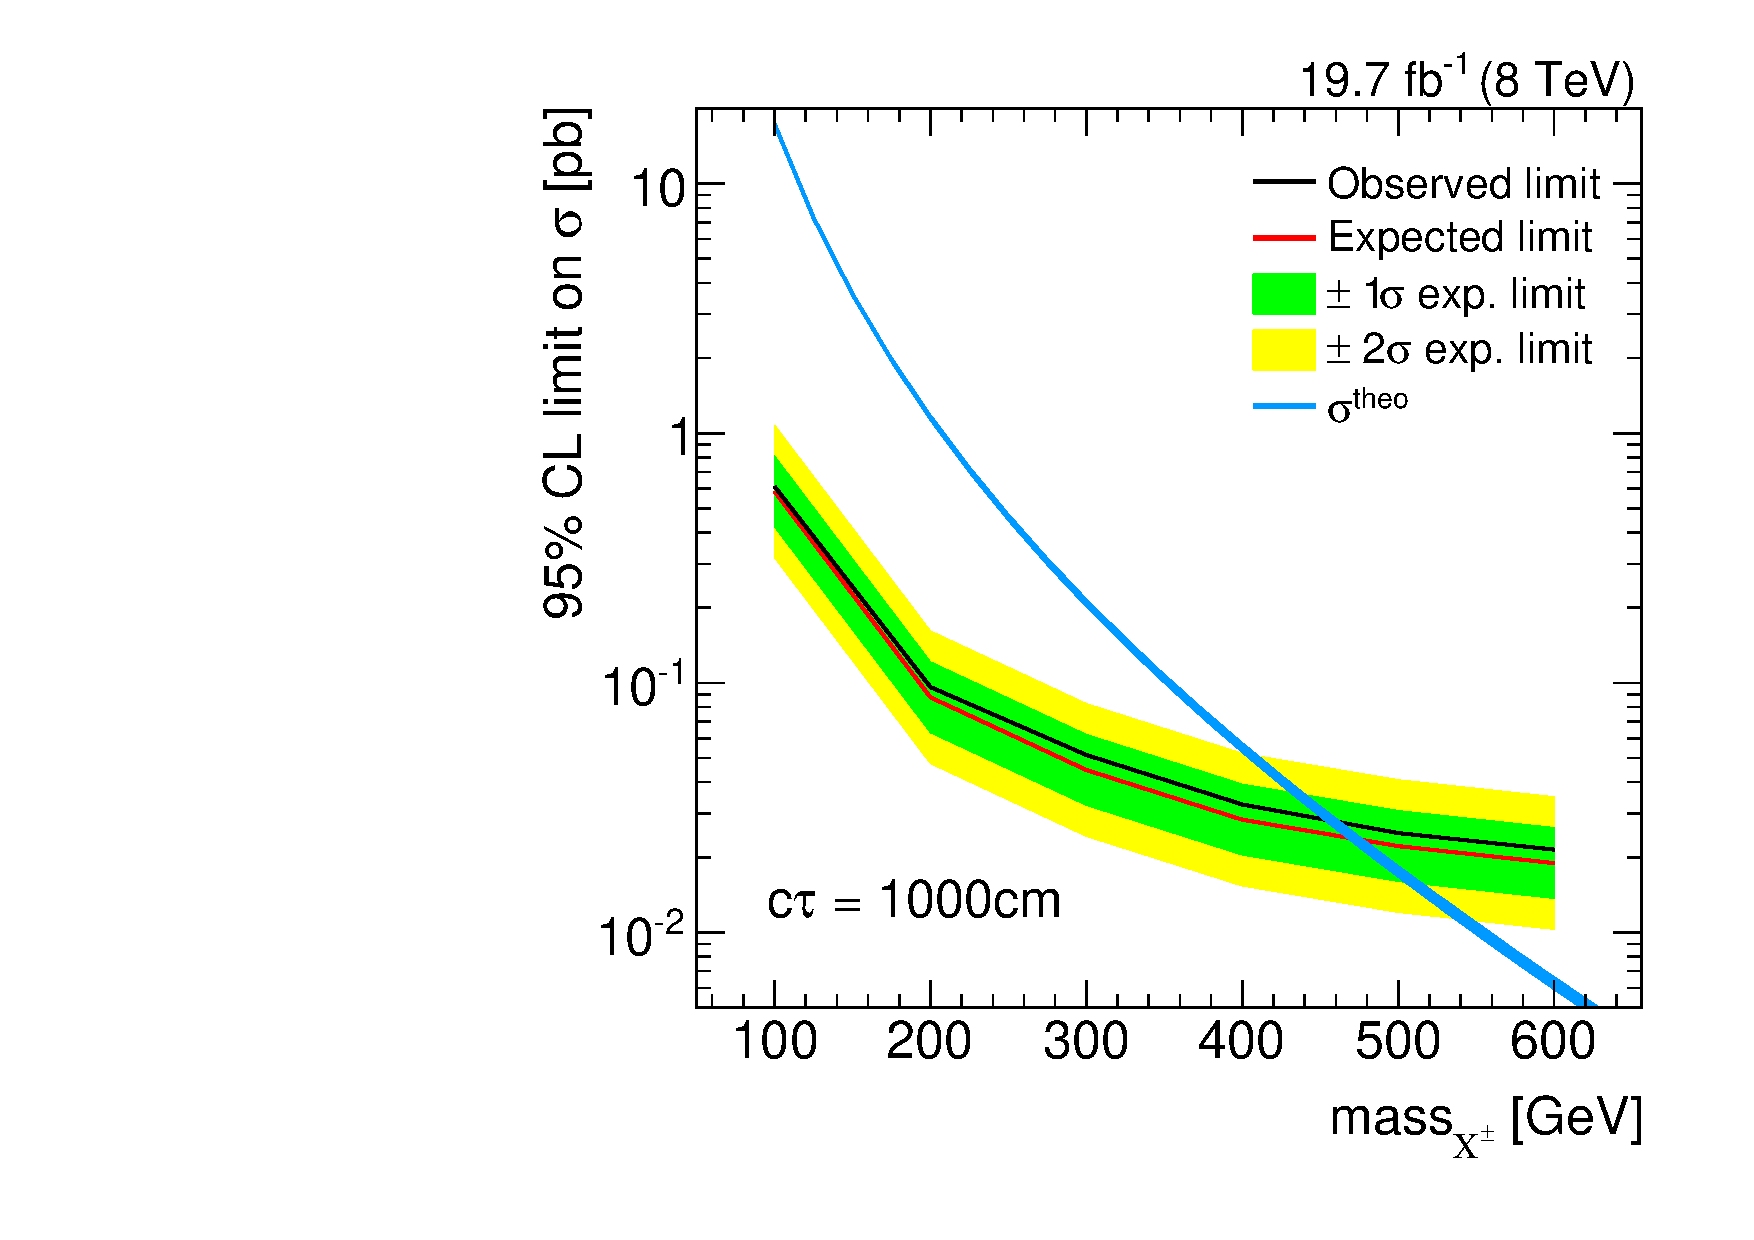
\includegraphics[width=0.49\textwidth]{figures/analysis/Interpretation/ExclusionLimits/LimitPlot_ctau1000cm.pdf} 
  \end{tabular}
  \caption{Four different \CLs exclusion limits for charginos with mean lifetimes of 5\cm (top left), 10\cm (top right), 50\cm (bottom left), 1000\cm (bottom right).
           The red line depicts the expected 95\% confidence level (CL) upper cross-section limit with the 1-$\sigma$ (green band) and 2-$\sigma$ (yellow band) intervals.
           The black line is the observed limit.
           The signal cross section is depicted as a blue line. 
           SUSY models can be excluded at 95\% CL if the signal cross section is at least as large as the 95\% CL observed upper limit on the cross section.}
  \label{fig:1dLimits}
\end{figure} 
The upper 95\% confidence level (CL) limit on the signal cross section is strongest for lifetimes between $10-100\cm$.
For lower lifetimes a sizable fraction of the charginos already decay before reaching the tracker.
For longer lifetimes, the cross section upper limit gets weaker again because the charginos start to be reconstructed as muons and do not pass the muon veto.
Also, the \ecalo requirement rejects these charginos with higher efficiency.

Due to the falling spectrum of the chargino production cross section, charginos with lower masses are more effectively excluded than charginos with higher masses.
A 2-dimensional exclusion limit in the chargino lifetime-mass parameter space is shown in Fig.~\ref{fig:2dLimit}.
\begin{figure}[!t]
  \centering 
  \begin{tabular}{c}
    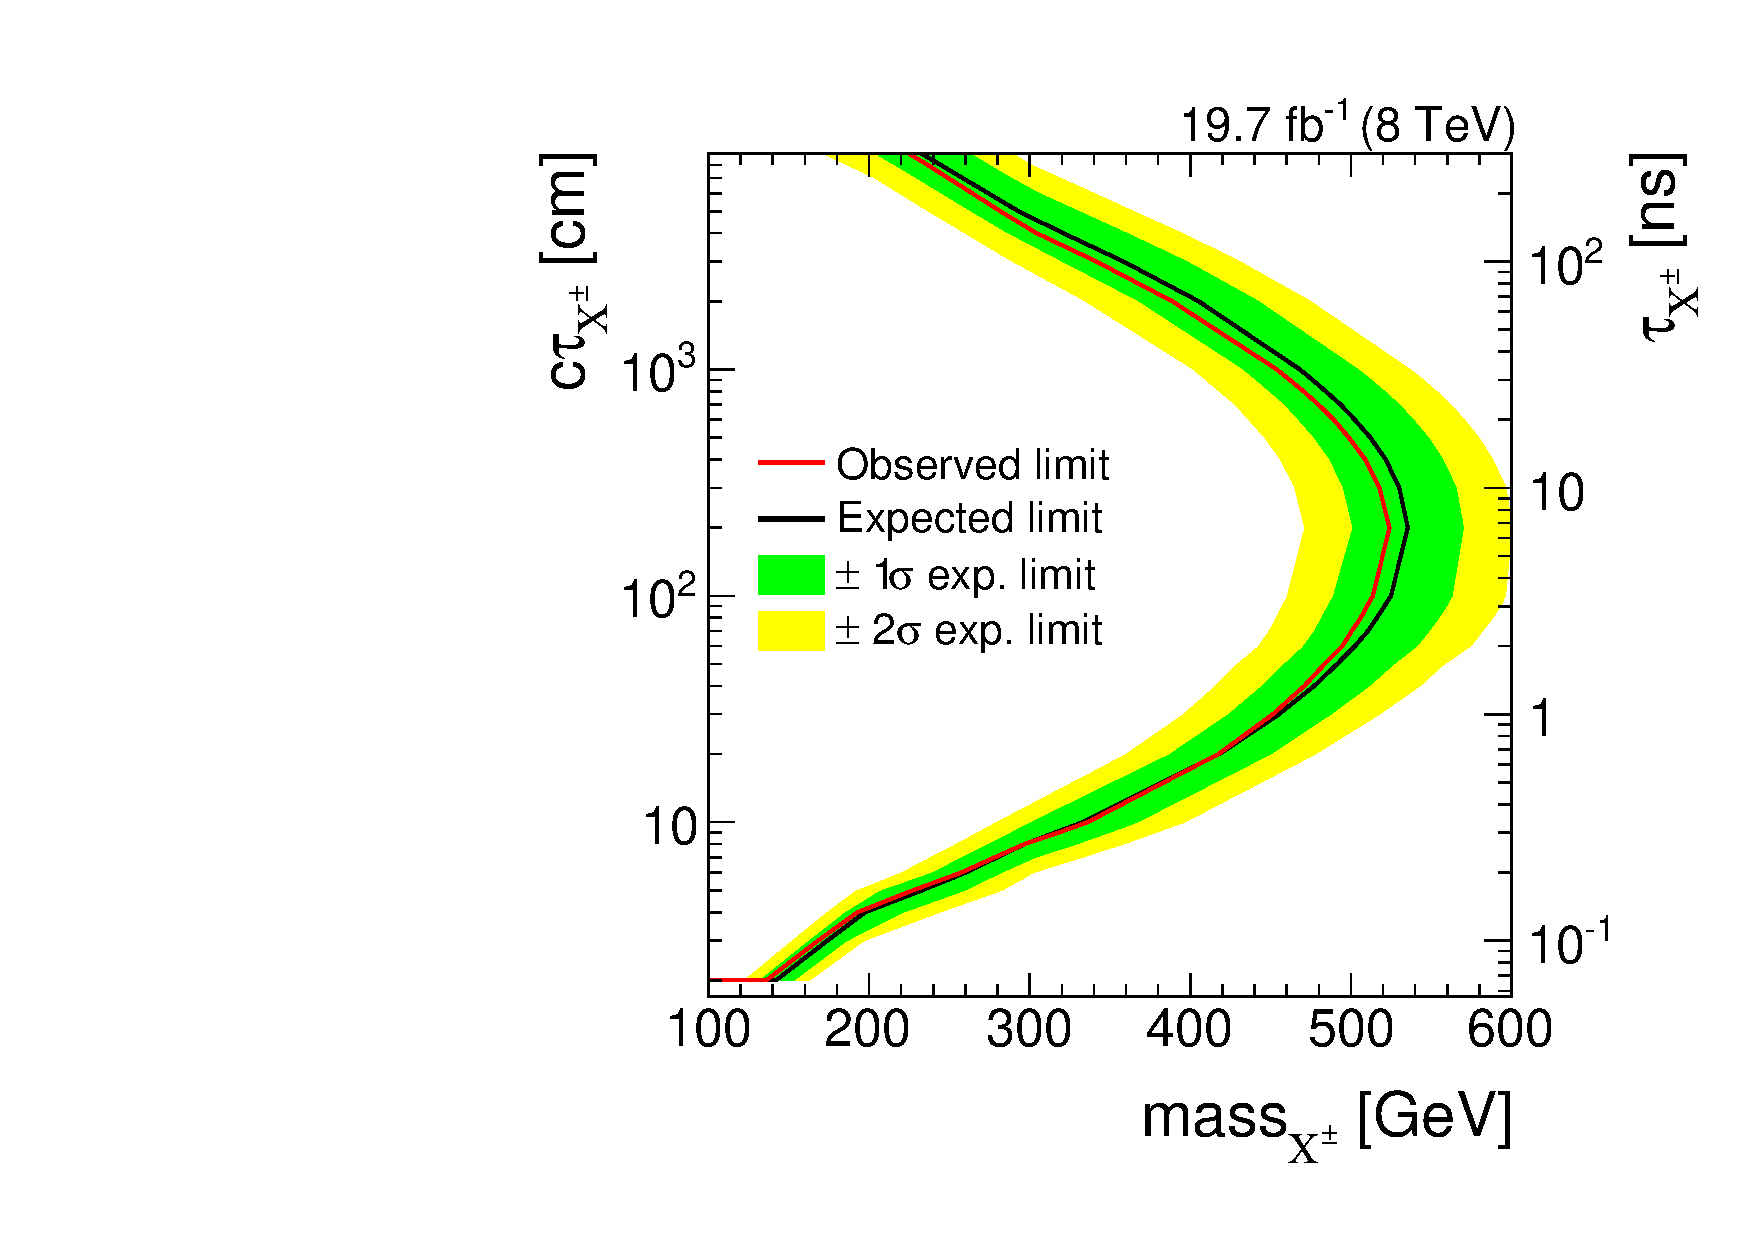
\includegraphics[width=0.79\textwidth]{figures/analysis/Interpretation/ExclusionLimits/LimitPlot_2d_log_cm.pdf} 
  \end{tabular}
  \caption{Excluded regions in the mass versus lifetime space.
           All excluded models are located left of the contour line.
            The red line depicts the expected 95\% CL upper cross-section limit with the 1-$\sigma$ (green band) and 2-$\sigma$ (yellow band) intervals.
           The black line is the observed limit.}
  \label{fig:2dLimit}
\end{figure} 

Charginos with masses of 100\gev can be excluded down to a lifetime of $\ctau=2\cm$.
Charginos with a higher mass of 500\gev are excluded for lifetimes between $\ctau=70-500\cm$.

Since the lifetime of a wino-like chargino is determined by the mass splitting between $m_{\chipm}$ and $m_{\chiO}$, 
it is possible to express the lifetime of the chargino as a mass gap $\Delta m_{\chipm\chiO}$ between the chargino and the lightest neutralino.
The correspondence between lifetime and mass gap is taken from~\cite{bib:MassSplitting_Drees}, where the decay width of $\chipm \rightarrow \chiO\, \pi^{\pm}$ is expressed in terms of chargino, neutralino, and pion mass.
Thus, the mass gaps that are considered are bounded by the pion mass of $\sim140\mev$.
The corresponding 2d exclusion limit can be found in Fig.~\ref{fig:DeltaMLimit2d}.
\begin{figure}[!t]
  \centering 
  \begin{tabular}{c}
    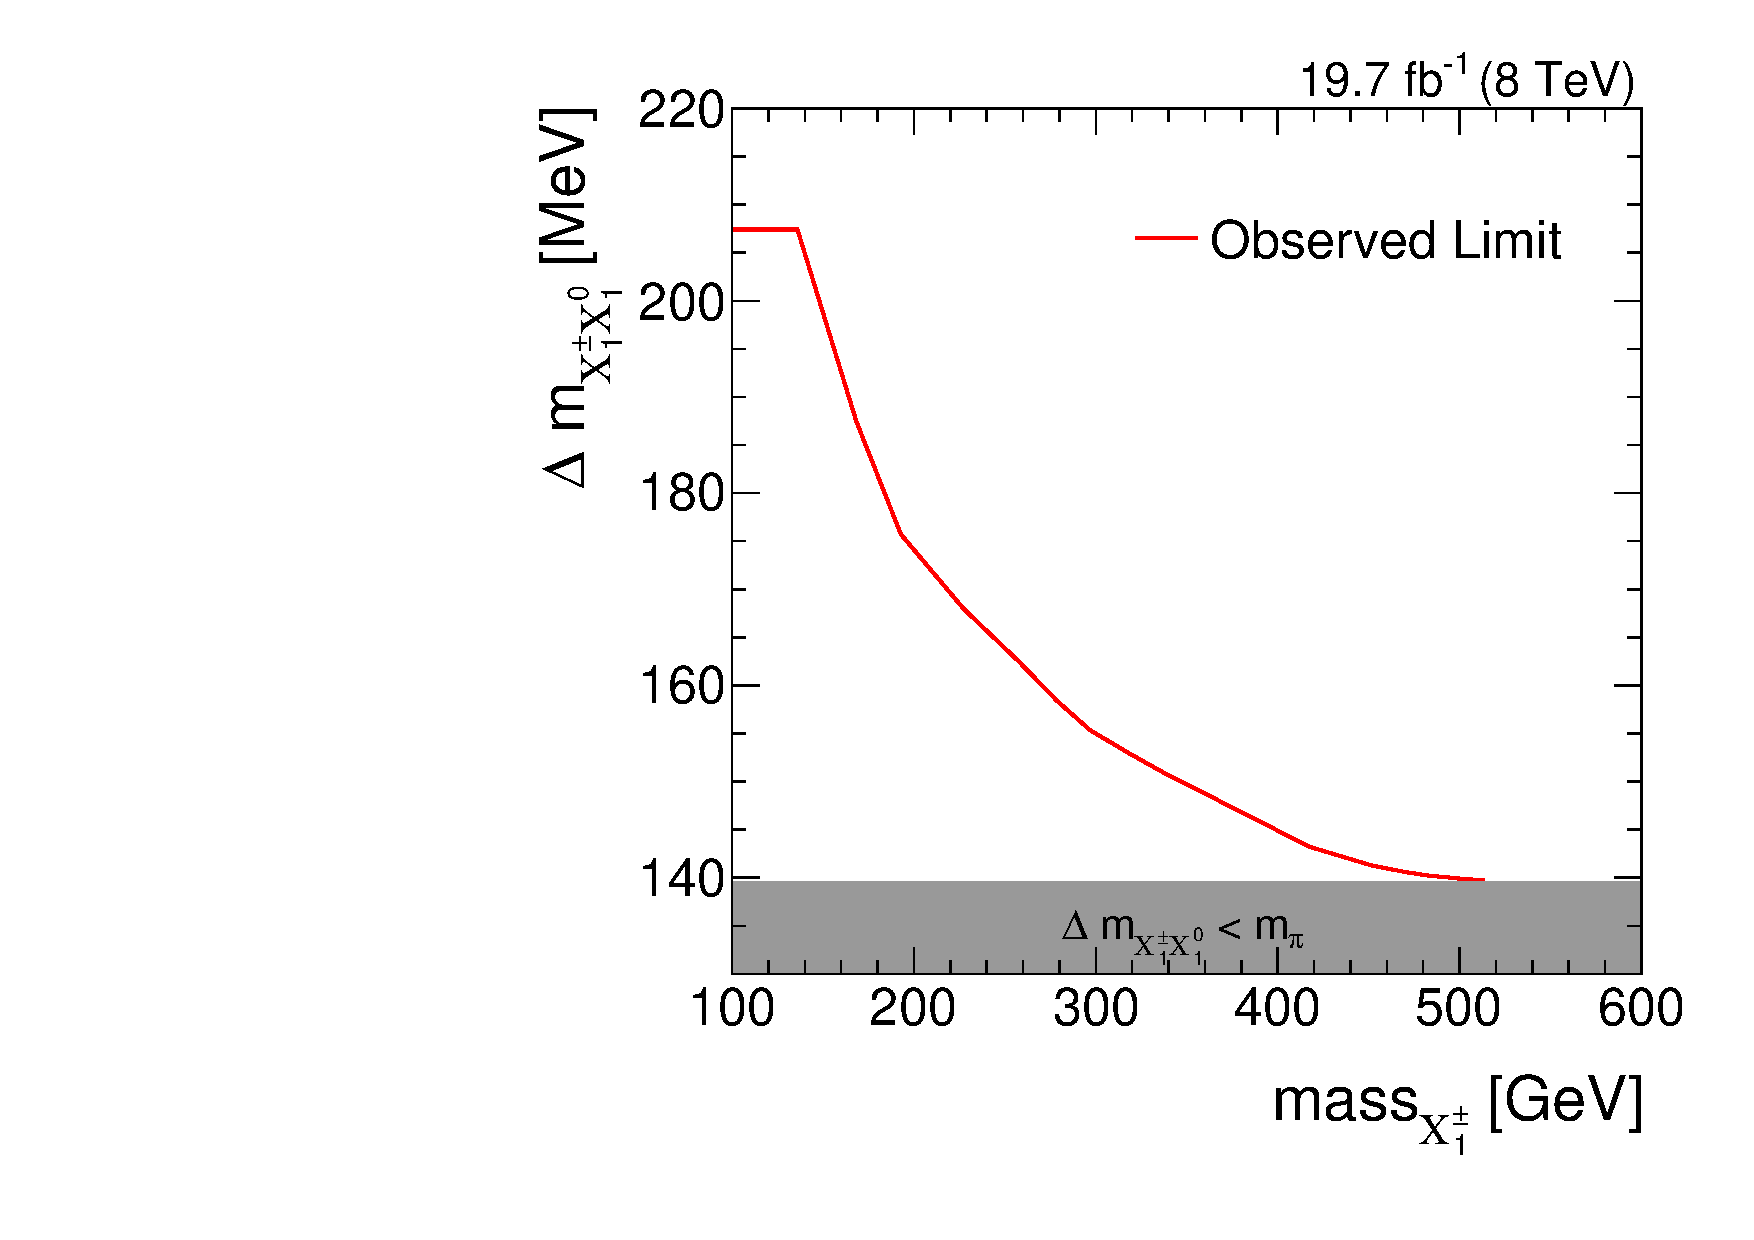
\includegraphics[width=0.55\textwidth]{figures/analysis/Interpretation/MassSplittingLimitPlot.pdf} 
  \end{tabular}
  \caption{Excluded parameter region at 95\% CL for wino-like charginos and neutralinos depending on the chargino mass and the mass splitting between \chipm and \chiO, $\Delta m_{\chipm\chiO}$.
          All SUSY models between the red line and the grey area are excluded.}
  \label{fig:DeltaMLimit2d}
\end{figure} 
It can be seen that this search is sensitive to mass splittings between $\sim 140\mev-210\mev$.\\

The presented exclusion limits confirm the exclusion from the search for disappearing tracks~\cite{bib:CMS:DT_8TeV} with slight improvements in the low lifetime region.
The comparison of the two searches is shown in Fig~\ref{fig:Comparison2dLimit}.

For charginos with a lifetime of $\tau=0.07\ns$ ($\ctau=2.1\cm$), the observed limit of this search improves the limits derived in~\cite{bib:CMS:DT_8TeV} by $\sim35\gev$ in chargino mass, for a lifetime of $\tau=0.4\ns$ ($\ctau=12.0\cm$) by $\sim25\gev$. 
For SUSY models with long chargino lifetimes the here presented search shows a higher exclusion power.
The weaker exclusion for long lifetimes in~\cite{bib:CMS:DT_8TeV} is caused by the additional selection cut on the number of missing outer hits, $\nlostouter\geq3$.

The confirmation of the excluded parameter space in~\cite{bib:CMS:DT_8TeV} is especially interesting since the signal regions of the two searches are little correlated.
The correlation between simulated signal events, that pass the selection from~\cite{bib:CMS:DT_8TeV}, $N_A$, and the selection used in this analysis, $N_B$, can be estimated by the event overlap $\rho_{\text{corr}}$
\begin{equation*}
\rho_{\text{corr}} = \frac{N_{A\cap B}}{N_{A \cup B}} = \frac{N_{A\cap B}}{N_A + N_B - N_{A \cap B}}.
\end{equation*}
In order to avoid an over- or underestimation of the event overlap, only the most sensitive signal region from this search is included in $N_B$.
The degree of correlation is depicted in Fig.~\ref{fig:AnalysisOverlap} which shows the event overlap for signal models with chargino masses between $100-600\gev$ and lifetimes between $5\cm-1000\cm$.
\begin{figure}[!t]
  \centering 
  \begin{tabular}{c}
    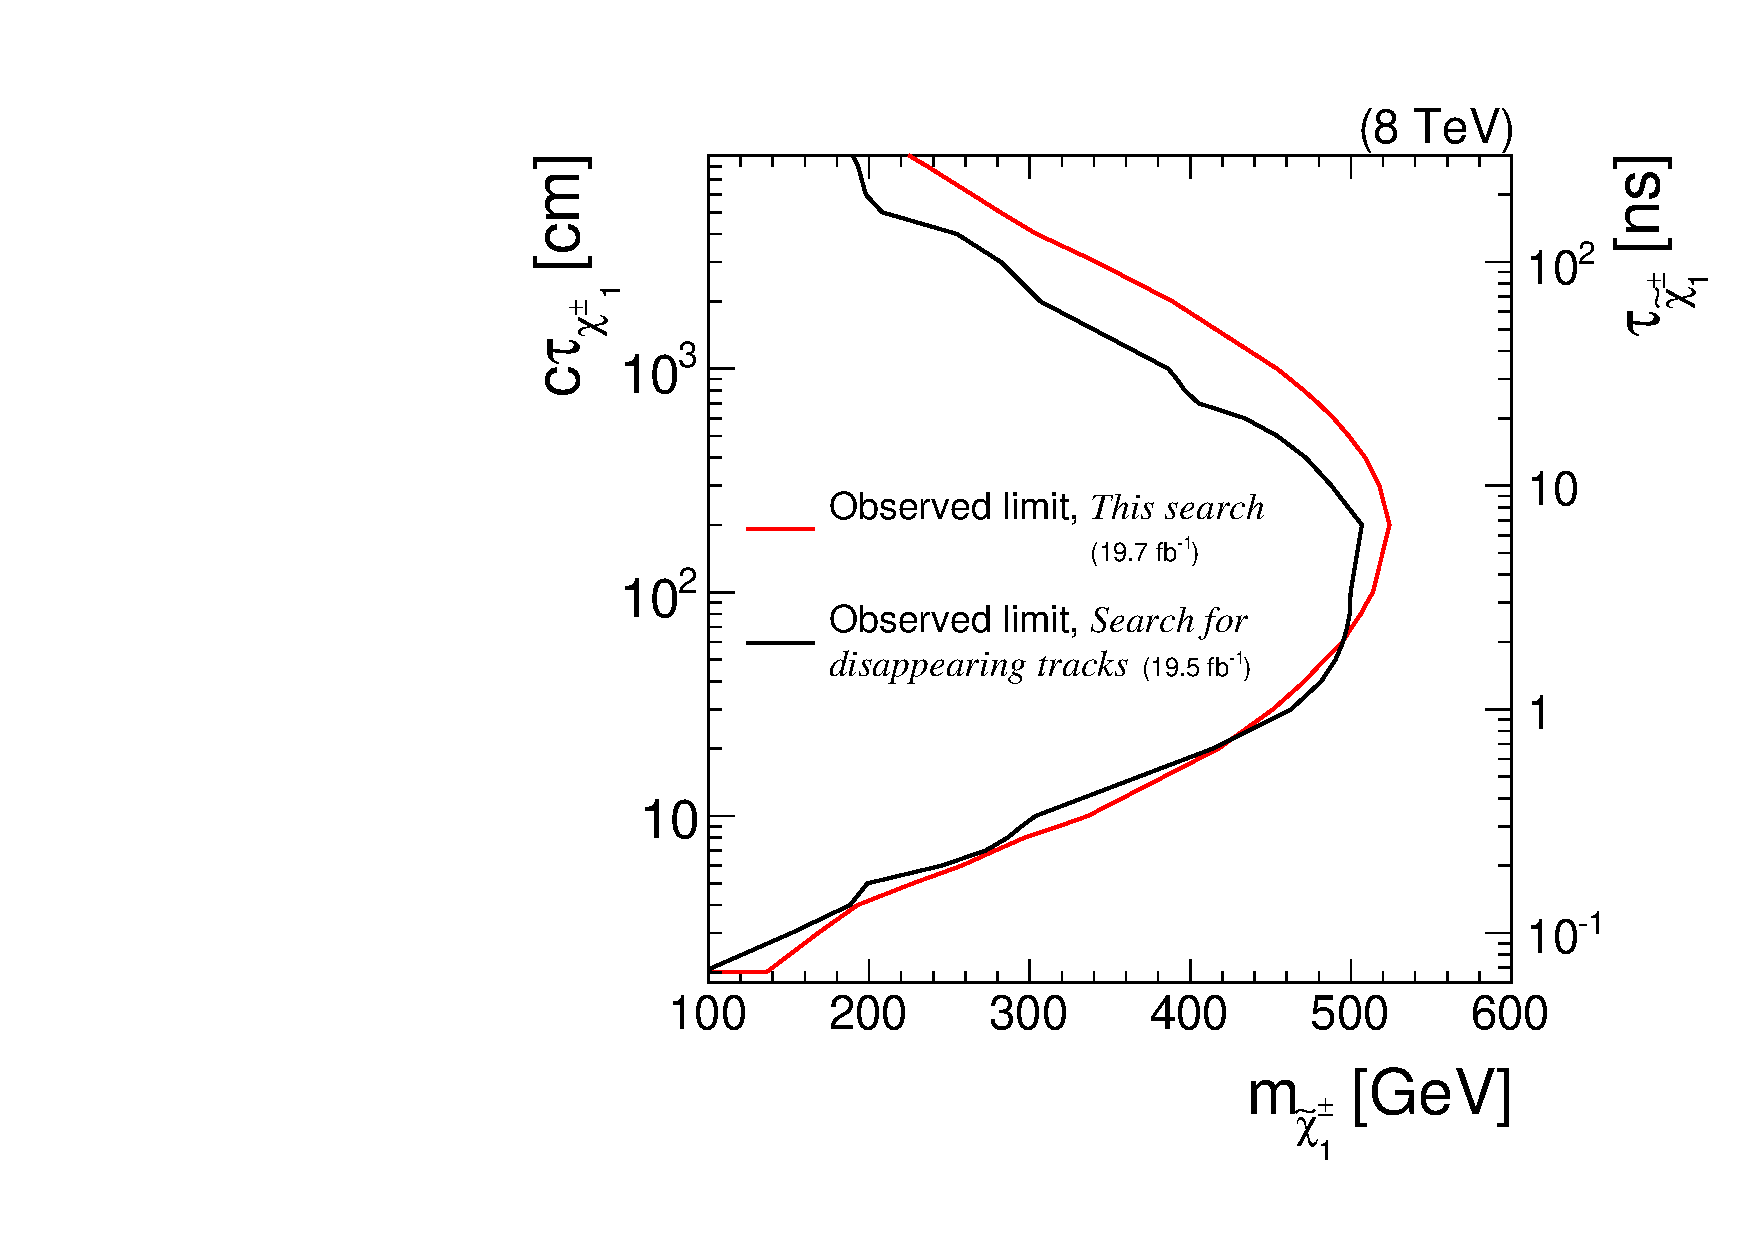
\includegraphics[width=0.49\textwidth]{figures/analysis/Interpretation/Comparison2dLimits_largerRange.pdf}  
    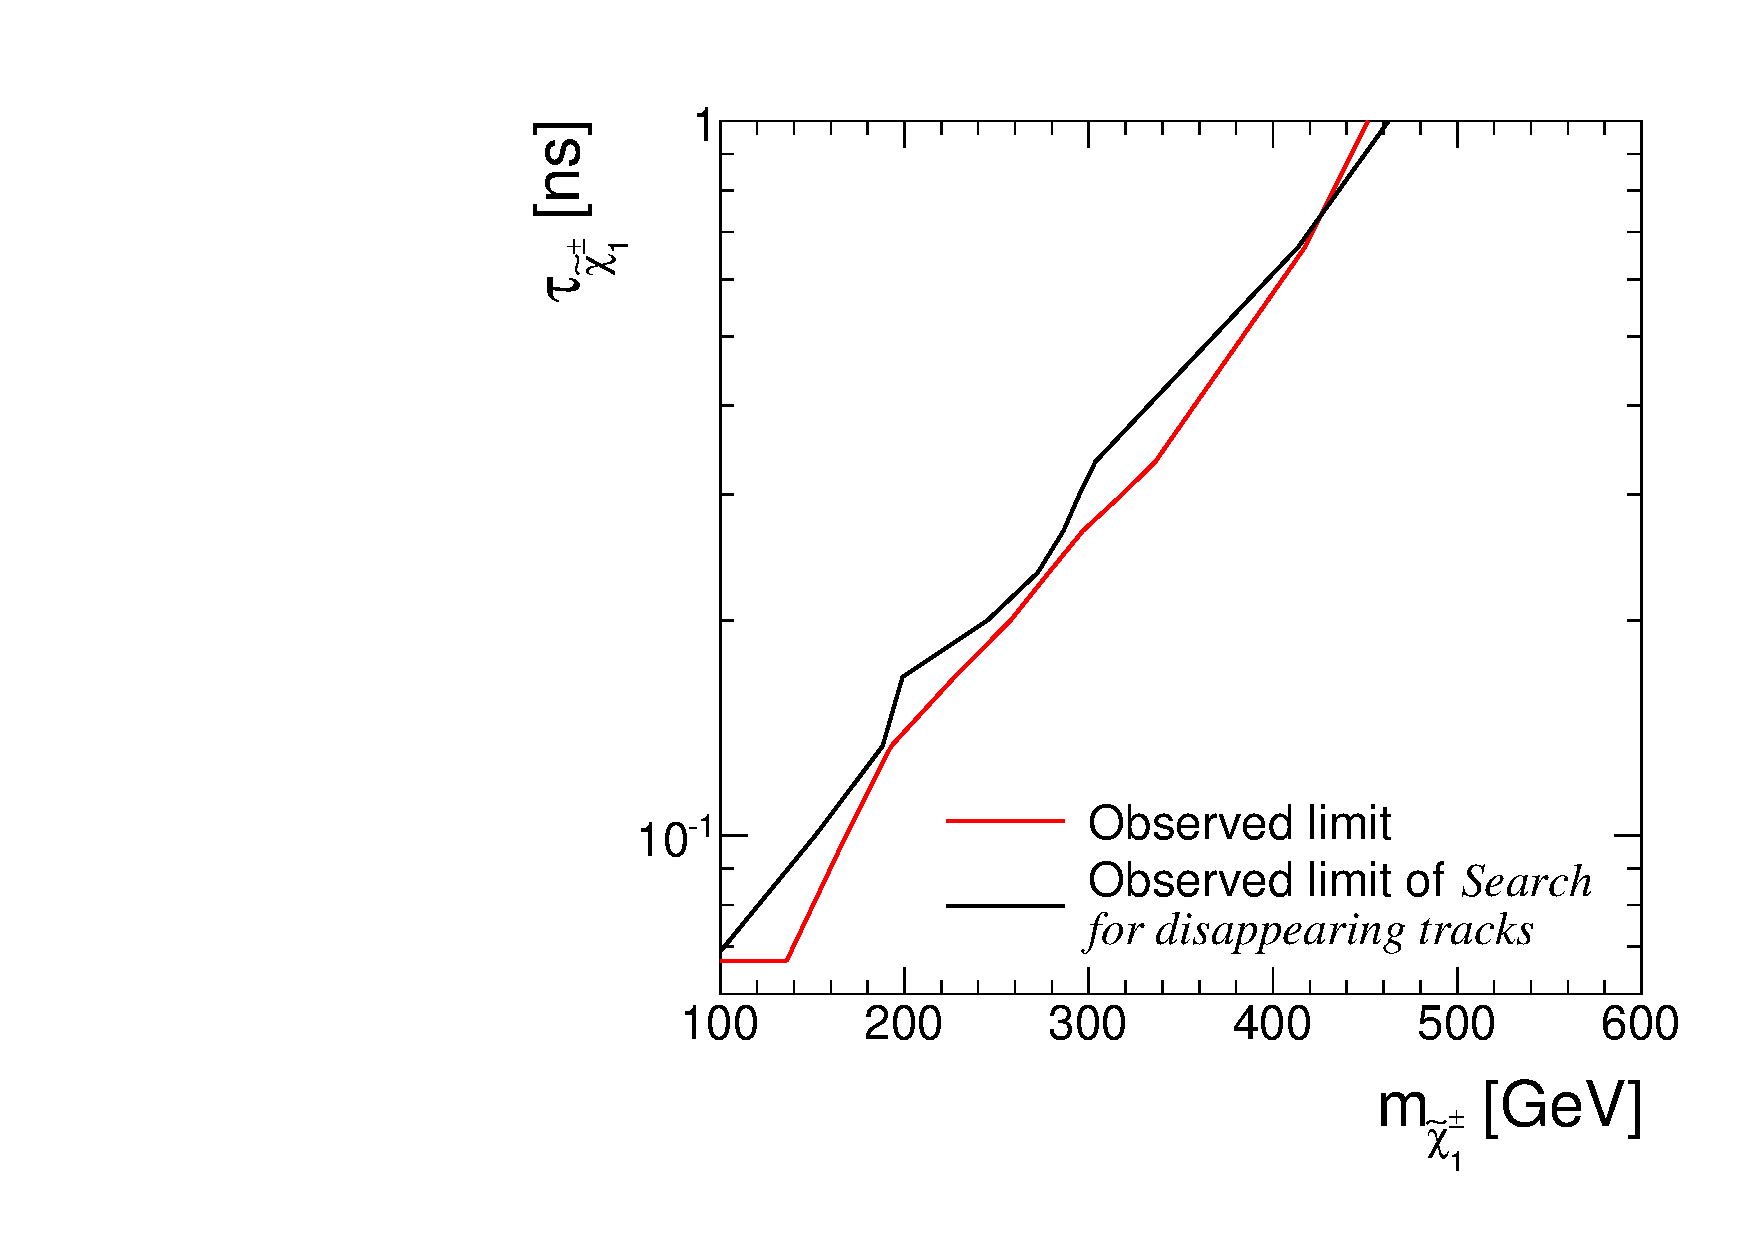
\includegraphics[width=0.49\textwidth]{figures/analysis/Interpretation/Comparison2dLimits.pdf} 
  \end{tabular}
  \caption{Comparison of the excluded regions in the mass versus lifetime space in this analysis (red line) and the search for disappearing tracks~\cite{bib:CMS:DT_8TeV} (black line). 
           The right figure is a zoom on the low lifetime region. All SUSY models left of the lines are excluded.}
  \label{fig:Comparison2dLimit}
\end{figure} 
\begin{figure}[!b]
\vspace{20pt}
  \centering 
  \begin{tabular}{c}
    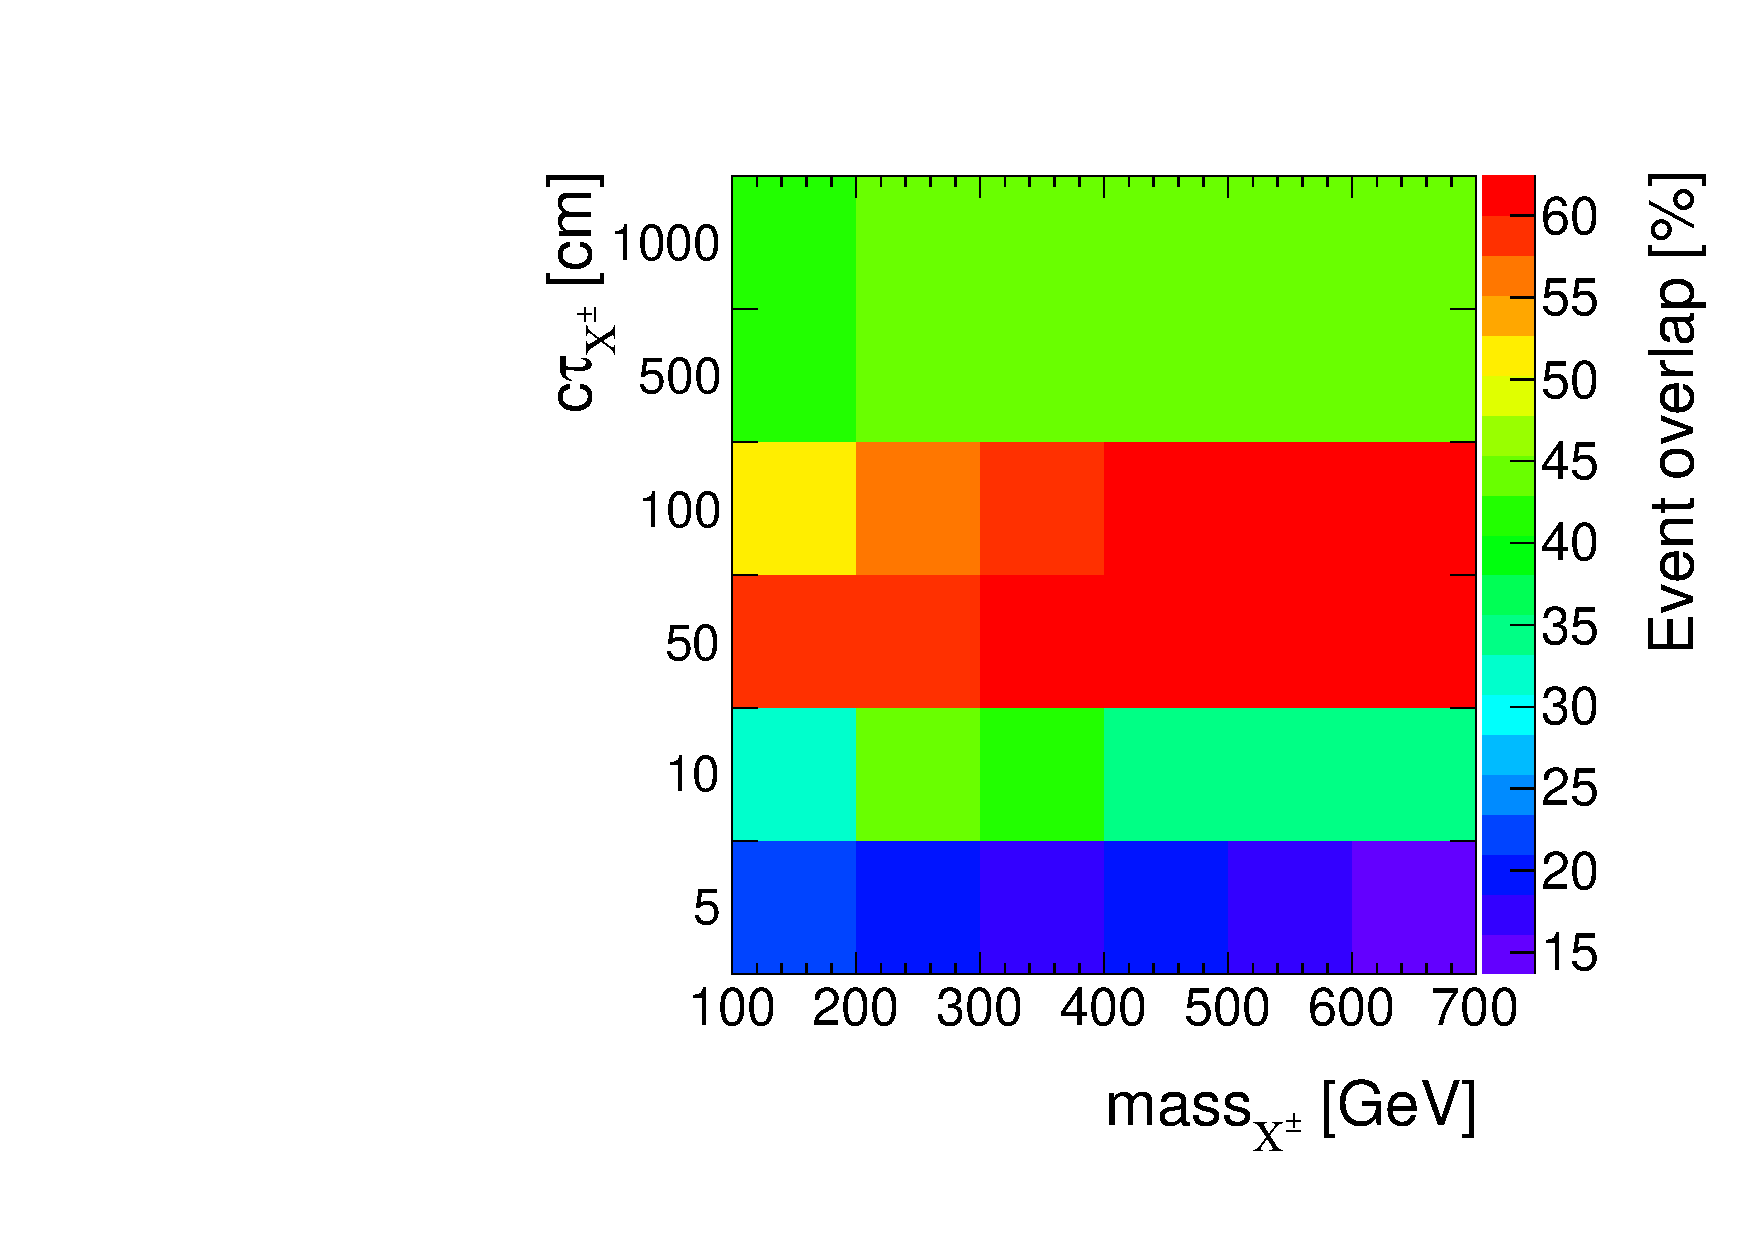
\includegraphics[width=0.49\textwidth]{figures/analysis/Interpretation/AnalysisOverlap.pdf}  
  \end{tabular}
  \caption{The event overlap between simulated signal events, that pass the selection from~\cite{bib:CMS:DT_8TeV} and the selection used in this analysis for different signal models.
          The correlation is determined using only the signal region with the highest sensitivity of this analysis.}
  \label{fig:AnalysisOverlap}
\end{figure} 
It can be seen that the event overlap for intermediate lifetimes of around 100\cm is around 60\% and decreases for shorter lifetimes to small overlaps of around $15-20\%$.
Additionally, the two events that were observed in data by~\cite{bib:CMS:DT_8TeV} in their signal region are not contained in any of the signal regions in the here presented analysis.
Thus, this analysis constitutes an independent confirmation of the exclusion limits derived in~\cite{bib:CMS:DT_8TeV}.

% with an almost independent set of simulated signal events for low lifetimes.
%It should also be noted that the two events observed in data in the signal region of~\cite{bib:CMS:DT_8TeV}, are not contained in any of the signal regions in the here presented analysis.
%One event is rejected by the tighter calorimeter isolation requirement of $\ecalo<5\gev$ (cf.~\cite{bib:CMS:DT_8TeV} required $\ecalo<10\gev$), and the other event is rejected by the stronger QCD suppression requirements.
%Thus, also the observed data shows no event overlap between this search and the search from~\cite{bib:CMS:DT_8TeV}.



%%%%%%%%%%%%%%%%%%%%%%%%%%%%%%%%%%%%%%%%%%%%%%%%%%%%%%%%%%%%%%%%%%%%%%%%%%%%%%%%%%%%%%%%%%%%%%%%%%%%%%%%%%%%%%%%%%%%%%%%%%%%%%%%%%%%%%%%%%%%%%%%%%%%%%%%%%%%%%%%%%%%%%%
%%%%%%%%%%%%%%%%%%%%%%%%%%%%%%%%%%%%%%%%%%%%%%%%%%%%%%%%%%%%%%%%%%%%%%%%%%%%%%%%%%%%%%%%%%%%%%%%%%%%%%%%%%%%%%%%%%%%%%%%%%%%%%%%%%%%%%%%%%%%%%%%%%%%%%%%%%%%%%%%%%%%%%%
